\documentclass[a4paper,oneside,czech,12pt]{book} % chcete-li si VÚ vytisknout, změňte "oneside" na "twoside"
%% === nezbytné balíčky:
%\usepackage[T1]{fontenc}
\usepackage[IL2]{fontenc}   % písmo pro UTF-8
\usepackage[utf8]{inputenc}    % vstupní znaková sada UTF-8
%\usepackage[cp1250]{inputenc}   % vstupní znaková sada: Windows 1250

\usepackage[czech]{babel} % česky psaná práce, typografická pravidla

\usepackage{rotating}
\usepackage{varioref}

%\usepackage{encxvlna} % postará se o spojky a předložky, které dle českých pravidel nesmí být na konci řádku. Dokumentace: http://texdoc.net/texmf-dist/doc/generic/encxvlna/encxvlna.pdf
\usepackage[a4paper, hmarginratio=2:2]{geometry} % využití celé A4 stránky a nastavení okrajů. Chcete-li si VÚ vytisknout, změňte: hmarginratio=3:2
\usepackage{pdfpages} % pokud nemáte formulář "Zadání VÚ" naskenovaný jako PDF, tak ZAKOMENTUJTE

%% === balíčky, které se mohou hodit:
\usepackage[hidelinks]{hyperref} % v PDF budou klikací odkazy ("hidelinks" je nebude rámovat)
\usepackage{graphicx} % balíček pro vkládání __rastrových__ grafických souborů (PNG apod.)
%\usepackage{epsfig} % balíčky pro vkládání grafických souborů typu EPS
%\usepackage{float} % rozšířené možnosti umístění obrázků

%\usepackage{caption} % pro popisky obrázků, tabulek atd.

\usepackage{tabularx} % rozšířené možnosti tabulek
%\usepackage{tabu} % jiný balík pro rozšířené možnosti tabulek

\usepackage{listings}  % balíček vhodný pro ukázky kódu 
\usepackage{amsmath} % balíček pro pokročilou matematickou sazbu
%\usepackage{color} % pro možnost barevného textu
%\usepackage{fancybox} % umožňuje pokročilé rámečkování

\usepackage{xcolor}

%\usepackage{index} % nutno použít v případě tvorby rejstříku balíčkem makeindex
%\newindex{default}{idx}{ind}{Rejstřík} % zavádí rejstřík v případě použití balíku index


\topmargin=-15mm      % horní okraj trochu menší
\textwidth=150mm      % šířka textu na stránce
\textheight=240mm     % "výška" textu na stránce

\frenchspacing % za větou bude mezislovní mezera (v anglických textech je mezera za větou delší)
\widowpenalty=1000 % "síla" zákazu vdov (= jeden řádek odstavce na konci stránky)
\clubpenalty=1000 % "síla" zákazu sirotků (= jeden řádek/slovo odstavce samostatně na začátku stránky)
\brokenpenalty=1000 % "síla" zákazu zlomu stránky za řádkem, který má na konci rozdělené slovo

\pagenumbering{arabic} % číslování stránek arabskými číslicemi
\pagestyle{plain}      % stránky číslované dole uprostřed

\parindent=0pt % odsazení 1. řádku odstavce
\parskip=7pt   % mezera mezi odstavci

\newcommand{\ti}{\textit} % zkrácený příkaz pro kurzívu
\newcommand{\tb}{\textbf} % zkrácený příkaz pro tučné písmo


%% --- zde jsou zavedeny některé "konstanty" - některé musíte změnit! --- %%
\newcommand{\cvut}{České vysoké učení technické v~Praze}
\newcommand{\fjfi}{Fakulta jaderná a fyzikálně inženýrská}
\newcommand{\ksi}{Katedra softwarového inženýrství}
\newcommand{\program}{Aplikace informatiky v~přírodních vědách} % změňte, pokud máte jiný stud. program
\newcommand{\specializace}{--} % změňte, pokud máte specializaci stud. programu

\newcommand{\druh}{Výzkumný úkol} % druh práce
\newcommand{\woman}{} % pokud jste ŽENA, ZMĚŇTE na: ...{\woman}{a} (je to do Prohlášení)

\newcommand{\logoCVUT}{
\includegraphics{symbol_cvut_konturova_verze_cb.pdf}} % logo ČVUT -- podle grafického manuálu ČVUT platného od prosince 2016. Pokud nevyhovuje PDF-verze, tak použijte jinou variantu loga: https://www.cvut.cz/logo-a-graficky-manual -> "Symbol a logo ČVUT v Praze"). Pokud chcete logo úplně vynechat, zadejte místo "\includegraphics{...}" text "\vspace{35mm}"

% přesně podle formuláře "Zadání VÚ" VYPLŇTE:
\newcommand{\nazevcz}{Vývoj strategické hry na náhodně generované mapě}    % český název práce (přesně podle zadání!)
\newcommand{\autor}{Bc. Štěpán Bezděk}   % vyplňte své jméno a příjmení (s akademickým titulem, máte-li jej)
\newcommand{\vedouci}{RNDr. Zuzana Petříčková, Ph.D.} % vyplňte jméno a příjmení vedoucího práce, včetně titulů, např.: Doc. Ing. Ivo Malý, Ph.D.
\newcommand{\pracovisteVed}{\ksi, \fjfi, \cvut} % ZMĚŇTE, pokud vedoucí Vaší práce není z KSI
\newcommand{\konzultant}{Ing. Vladimír Jarý, Ph.D.} % POKUD MÁTE určeného konzultanta, NAPIŠTE jeho jméno a příjmení
\newcommand{\pracovisteKonz}{Katedra softwarového inženýrství, Fakulta jaderná a fyzikálně inženýrská, ČVUT v Praze} % POKUD MÁTE konzultanta, NAPIŠTE jeho pracoviště

% podle skutečnosti VYPLŇTE:
\newcommand{\rok}{2025}  % rok odevzdání práce (jen rok odevzdání, nikoli celý akademický rok!)
\newcommand{\kde}{Praze}

\newcommand{\klicova}{Klíčová slova}   % zde NAPIŠTE česky max. 5 klíčových slov
\newcommand{\abstrCZ}{Popis VÚ česky}    % zde NAPIŠTE abstrakt v češtině (cca 7 vět, min. 80 slov)

\newcommand{\prohlaseni}{Prohlašuji, že jsem svůj výzkumný úkol vypracoval\woman{} samostatně a použil\woman{} jsem pouze podklady (literaturu, projekty, SW atd.) uvedené v přiloženém seznamu.} % text prohlášení můžete mírně upravit :-)

\newcommand{\podekovani}{Děkuji ... za ...} % NAPIŠTE poděkování, např. svému vedoucímu:
%"Děkuji Ing. Eleonoře Krtečkové, Ph.D. za vedení mého výzkumného úkolu a za podnětné návrhy, které jej obohatily."
% NEBO:
% Děkuji doc. Pafnutijovi Snědldítětikaši, Ph.D. za neocenitelné rady a pomoc při tvorbě výzkumného úkolu.


\begin{document}
%%%%%%%%%%%% TITULNÍ STRANA -- následujících cca 30 řádků se generuje AUTOMATICKY (není třeba nic měnit) %%%%%%%%%%%%
\thispagestyle{empty}

\begin{center}
    {\Large \textsc{\cvut}\\[1.5ex] \textsc{\fjfi}}\\
    \vspace{10mm}

    \begin{tabular}{ll}
		\multicolumn{2}{c}{\tb{\ksi}} \\[8pt]   
		\tb{Studijní program:} & \tb{\program}\\
		\tb{Specializace:} & \tb{\specializace}\\
    \end{tabular}

   \vspace{13mm} \logoCVUT \vspace{15mm} 

   {\huge \tb{\nazevcz}\par}
   \vspace{5mm}   
   
   \vspace{15mm}
   {\Large \MakeUppercase{\druh}}

   \vfill
   {\large
    \begin{tabular}{ll}
    Vypracoval: & \autor\\
    Vedoucí práce: & \vedouci\\
    Rok: & \rok
    \end{tabular}
   }
\end{center}

%%%%%%%%%%%% ZADÁNÍ PRÁCE %%%%%%%%%%%%
% Zadání (podepsané!) musíte NASKENOVAT. Ideálně jako jednostránkové PDF (soubor "zadaniVU.pdf"). 
%\newpage  % SEM NESAHEJTE!
\thispagestyle{empty} % SEM NESAHEJTE!

% --- varianta A: zadání naskenované jako 2stránkové PDF:
\includepdf[pages={1}]{Zadání_VÚ_Bezděk.pdf} % zadání naskenované jako PDF
%% --- varianta B: zadání naskenované jako obrázek (JPG):
%\begin{center}
%     \includegraphics[width=1\textwidth]{zadani1.jpg}
%\end{center}
%\newpage ~  % prázdná stránka za zadáním -- oboustranný tisk; SEM NESAHEJTE!
%\thispagestyle{empty} % SEM NESAHEJTE!


%%%%%%%%%%%% Prohlášení -- SEM NESAHEJTE! Generuje se automaticky z výše nastavených maker \kde{} a \prohlaseni{}. %%%%%%%%%%%%
\newpage % SEM NESAHEJTE!
\thispagestyle{empty}  % SEM NESAHEJTE!

~ % SEM NESAHEJTE!
\vfill % prázdné místo. SEM NESAHEJTE!

\tb{Prohlášení} % SEM NESAHEJTE!

\vspace{1em} % vertikální mezera. SEM NESAHEJTE!
\prohlaseni

\vspace{2em}  % SEM NESAHEJTE!
\hspace{-0.5em}\begin{tabularx}{\textwidth}{X c}  % SEM NESAHEJTE!
V \kde\ dne .................... &........................................ \\	% SEM NESAHEJTE!
	& \autor
\end{tabularx}	% SEM NESAHEJTE!


%%%%%%%%%%%% Poděkování -- tuto stránku můžete celou odstranit %%%%%%%%%%%%
\newpage
\thispagestyle{empty}

~
\vfill % prázdné místo

\tb{Poděkování}

\vspace{1em} % vertikální mezera
\podekovani
\begin{flushright}
\autor
\end{flushright}  % <-- konec stránky s poděkováním


%%%%%%%%%%%% ABSTRAKT atp. Je generován AUTOMATICKY podle maker nastavených na začátku souboru) %%%%%%%%%%%% 
\newpage   % SEM NESAHEJTE!
\thispagestyle{empty}   % SEM NESAHEJTE!

% příprava:    (na následujících 8 řádků NESAHEJTE!)
\newbox\odstavecbox
\newlength\vyskaodstavce
\newcommand\odstavec[2]{%
    \setbox\odstavecbox=\hbox{%
         \parbox[t]{#1}{#2\vrule width 0pt depth 4pt}}%
    \global\vyskaodstavce=\dp\odstavecbox
    \box\odstavecbox}
\newcommand{\delka}{120mm} % šířka textů ve 2. sloupci tabulky

% použití přípravy:    % dovnitř "tabular" vůbec NESAHEJTE!
\begin{tabular}{ll}
  {\em Název práce:} & ~ \\
  \multicolumn{2}{l}{\odstavec{\textwidth}{\bf \nazevcz}} \\[1em]
  {\em Autor:} & \autor \\[1em]
  {\em Studijní program:} & \program \\
  {\em Specializace:} & \specializace\\
  {\em Druh práce:} & \druh \\[1em]
  {\em Vedoucí práce:} & \odstavec{\delka}{\vedouci\\ \pracovisteVed} \\
  {\em Konzultant:} & \odstavec{\delka}{\konzultant \\ \pracovisteKonz}  % VYMAŽTE text "-- %" v případě, že jste neměli konzultanta
 \\[1em]  
  \multicolumn{2}{l}{\odstavec{\textwidth}{{\em Abstrakt:} ~ \abstrCZ  }} \\[1em]
  {\em Klíčová slova:} & \odstavec{\delka}{\klicova}
\end{tabular}



%%%%%%%%%%%% Obsah VÚ ... je generován AUTOMATICKY %%%%%%%%%%%%
\parskip=0pt
\tableofcontents % SEM NESAHEJTE!
\parskip=7pt
%\newpage % SEM NESAHEJTE!


%--------------------------------------------------------
%|         Zde začíná SAMOTNÁ PRÁCE (text)              |
%--------------------------------------------------------

\chapter*{Úvod} % SEM NESAHEJTE!
\addcontentsline{toc}{chapter}{Úvod} % SEM NESAHEJTE!
%
Zde napište text úvodu (1-3 strany, nerozdělujte na podkapitoly) nebo jej vložte ze samostatného souboru: např. příkazem \texttt{\textbackslash input\{uvod.tex\}}.

Tato šablona je určena {\color{red}pro elektronické odevzdání VÚ} (od roku 2023). Pokud byste si VÚ chtěli vytisknout, tak změňte řádky~1~a~10 ve zdrojovém kódu této šablony ($\Rightarrow$ budou správně nastavené \uv{prázdné zadní stránky}).
%
%\input{uvod.tex}


\chapter{Teorie PCG}
\definecolor{darkgreen}{rgb}{0.0, 0.5, 0.0}
\lstdefinestyle{mystyle}{
    backgroundcolor=\color{white}, % pozadí kódu
    commentstyle=\color{green},
    keywordstyle=\color{blue},
    numberstyle=\tiny\color{gray},
    stringstyle=\color{darkgreen},
    basicstyle=\ttfamily\footnotesize,
    breakatwhitespace=false,
    breaklines=true,
    captionpos=b,
    keepspaces=true,
    numbers=left,
    numbersep=5pt,
    showspaces=false,
    showstringspaces=false,
    showtabs=false,
    tabsize=2,
    frame=single,
}
\lstset{style=mystyle}
% Změna textu "Listing" na "Ukázka"
\renewcommand\lstlistingname{Ukázka}
\renewcommand\lstlistlistingname{Ukázky kódu}

\section{Procedurální generování obsahu (PCG)}

Zpracováno na základě: \cite{PCGinG} \cite{HistoryOfPCG}.

Procedurální generování je metoda algoritmického vytváření dat. Procedurálně vytvořená data se od ručně vytvořených dat liší v tom, že jsou generována kombinací malého množství ručně vytvořených vstupních dat, na jejichž základě počítač podle daného algoritmu vytváří komplexnější výstup. Tento přístup je vhodný zejména pro aplikace, kde je vyžadováno velké množství různorodého obsahu nebo kde je ruční tvorba neefektivní.

Hlavní výhodou procedurálního generování je úspora času, lidských zdrojů a tím i finančních nákladů. Navíc umožňuje vytvořit obsah, který může být přizpůsoben konkrétním požadavkům nebo preferencím uživatele. Generovaný obsah je dynamický, což otevírá možnosti pro personalizaci zážitků, jako je například tvorba jedinečných map ve hrách nebo simulace náhodných prostředí.

\subsection{Výhody procedurálního generování}
Procedurální generování nabízí mnoho výhod, které ho činí atraktivním pro různé aplikace, hlavně ve vývoji her a designu:
\begin{itemize}
    \item \textbf{Redukce nároků na úložiště:} Namísto ukládání velkého množství dat je možné ukládat pouze algoritmus a jeho vstupní parametry.
    \item \textbf{Variabilita:} Algoritmus může generovat nekonečné množství unikátních výsledků.
    \item \textbf{Dynamika:} Obsah se může přizpůsobovat v reálném čase na základě uživatelských interakcí nebo jiných faktorů.
    \item \textbf{Úspora lidských zdrojů:} Omezuje potřebu ruční práce při tvorbě rozsáhlých prostředí.
\end{itemize}

\subsection{Nevýhody a výzvy procedurálního generování}
Ačkoliv má procedurální generování mnoho výhod, existují také určité nevýhody a výzvy:
\begin{itemize}
    \item \textbf{Kontrola kvality:} Výstup algoritmu nemusí vždy splňovat očekávání nebo být konzistentní s požadovanými normami.
    \item \textbf{Složitost implementace:} Návrh a ladění algoritmů mohou být časově náročné.
    \item \textbf{Předvídatelnost:} Přílišná náhodnost může vést k obsahu, který nedává smysl nebo není použitelný.
    \item \textbf{Závislost na vstupních datech:} Kvalita výstupu je silně ovlivněna kvalitou a rozmanitostí vstupních dat.
\end{itemize}

\subsection{Procedurální generování ve hrách}

Kapitola zpracována s~pomocí: \cite{PCGinG} \cite{HistoryOfPCG}.

Procedurální generování obsahu hraje klíčovou roli v moderním herním vývoji, zejména díky schopnosti efektivně vytvářet rozsáhlé a rozmanité herní světy. Tento přístup je oblíbený především pro hry s otevřeným světem, jako jsou \emph{Minecraft}, \emph{No Man's Sky} nebo série \emph{Rogue-like} her, kde je kladen důraz na variabilitu a dynamické prostředí.

Procedurální generování umožňuje vytvořit herní světy, které jsou pro hráče vždy jedinečné, což zvyšuje atraktivitu a prodlužuje životnost hry. Například v \emph{Minecraftu} se každý nový svět skládá z unikátní kombinace biomů, terénních útvarů a zdrojů, což hráče motivuje k dalšímu průzkumu. Podobně ve hře \emph{No Man's Sky} je generován celý vesmír s miliardami planet, z nichž každá má unikátní prostředí, faunu a flóru.

Hlavní výhodou využití PCG v herním designu je schopnost generovat obsah přizpůsobený hráčově zkušenosti. Například v akčních hrách mohou algoritmy procedurálního generování upravovat obtížnost úrovní v reálném čase na základě výkonu hráče. Tento adaptivní přístup může zajistit, že hra zůstane náročná, ale zároveň nefrustrující, což zvyšuje angažovanost hráče.

Dalším využitím PCG je tvorba náhodných misí nebo úkolů. Ty mohou být generovány tak, aby obsahovaly různé cíle, nepřátele nebo interaktivní objekty. Tento přístup umožňuje vytvořit dynamický herní zážitek, kdy žádná mise nebo průběh hry nejsou zcela stejné. Tento princip se často využívá například ve hrách typu \emph{Diablo} nebo \emph{Borderlands}, kde jsou zbraně a další vybavení generovány procedurálně.

I přes četné výhody s sebou procedurální generování přináší i určité výzvy. Například ve hře \textit{No Man's Sky} čelili vývojáři kritice za přílišnou repetitivnost obsahu, přestože byl generován procedurálně. Dalším problémem je zajištění smysluplnosti a konzistence herního světa, což vyžaduje pečlivě navržené algoritmy a pravidla.

\subsubsection{Procedurální generování textur a zvuků}
Procedurální generování nachází své uplatnění také při tvorbě textur a zvuků, což významně přispívá k redukci nároků na úložný prostor. Textury povrchů, jako jsou dřevo, kámen nebo kov, mohou být generovány pomocí algoritmů, jako je \textbf{Perlin Noise} nebo \textbf{Simplex Noise}. Také je tímto přístupem možné generovat vegetaci, tak aby každý strom a keř vypadal unikátně například pomocí \textbf{Grammar Algorithms}. Tento přístup nejen šetří místo na disku, ale také zvyšuje variabilitu, protože každá textura může být jedinečná.

Podobně lze procedurálně generovat zvuky, jako je ambientní hudba nebo efekty prostředí (například šum deště, větru či zvuky zvířat). Použitím technik syntézy zvuku místo ukládání statických zvukových souborů je možné dynamicky přizpůsobit zvukové efekty aktuálním podmínkám ve hře, čímž se nejen šetří úložiště, ale také zlepšuje ponoření hráče do herního prostředí.


\section{Metody procedurálního generování map}

V rámci této práce využijeme procedurální generování specificky pro vytvoření nové herní plochy pro každou hru. V této části se podíváme na některé možné techniky pro generování herních map. Hlavními požadavky na algoritmy jsou logické rozložení mapy, hratelnost a rychlost generování.

Algoritmy byly mimo jiné zpracovány na základě: \cite{PCGinG}.

\subsection{Space Partitioning}

%Nepoužitý odkaz: https://gameprogrammingpatterns.com/spatial-partition.html

Dělení prostoru je metoda, která rekurzivně rozděluje herní mapu na menší, disjunktní oblasti, přičemž každý bod mapy náleží právě jedné z těchto oblastí. Výsledkem je hierarchická struktura, obvykle reprezentovaná stromem, která umožňuje rychlé vyhledávání informací a manipulaci s daty.

Hlavním principem této metody je postupné dělení základního prostoru, dokud nejsou splněny předem stanovené podmínky, jako je například minimální velikost buňky nebo místnosti. Tento přístup nachází uplatnění nejen při generování herních map, ale také v grafických aplikacích, jako je ray-tracing, kde umožňuje efektivně organizovat a vykreslovat objekty ve scéně. \cite{PCGclanek}.

Nejběžnější metoda pro rozdělování prostoru je \textit{binární dělení prostoru (BSP)}. Jde o proces, který opakovaně rozděluje prostor na dvě části, dokud nejsou splněny určité požadavky. Ukázka \textit{BSP} je zobrazena na obrázku \vref{BSP_ukazka}. Další často využívanou variantou je \textit{quadtree}, kde je prostor rozdělen na čtyři symetrické části. Hlavním rozdílem mezi \textit{quadtree} a \textit{BSP} je, že v \textit{BSP} nemusí být na rozdíl od \textit{quadtree} všechny buňky symetrické a buňky v \textit{BSP} navíc nemusí mít stejnou orientaci \cite{BSPclanek}.

Metoda je běžně využíváno při vykreslování grafických scén, kde se dělící roviny vybírají na základě polygonů, aby optimalizovaly výpočty. Pro renderování scény je například důležité zajistit, že každý uzel stromu obsahuje polygony, které lze vykreslit efektivně. \cite{BSPclanek}.

\begin{figure}
  \centering      % vycentrovat
  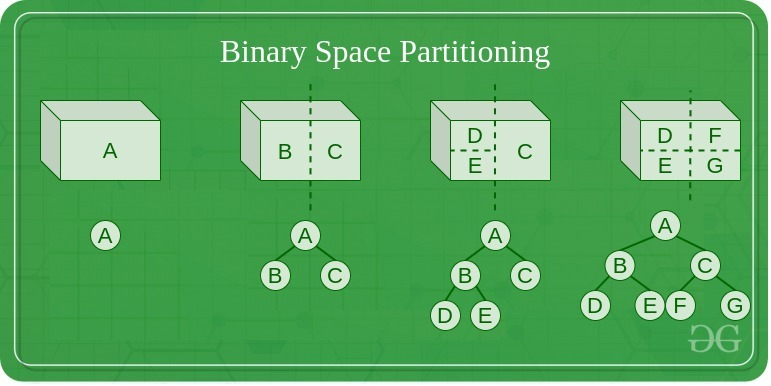
\includegraphics[scale=0.6]{obr/BSP.jpg} % soubor + měřítko (scale)
  \caption{Ukázka \textit{BSP} \cite{BSPclanek}} % popis obrázku
  \label{BSP_ukazka} % definice odkazu na obrázek (pro \ref{})
\end{figure}

\subsection{Agent-Based generování}
%Měl bych citovat každý odstavec když jsou všechny ze stejného zdroje?

Nejjednodušší \textit{agent-based} metoda přistupuje ke generování úrovní tak, že vygeneruje agenta, který "vykopává" chodby a vytváří oblasti v souvislé sekvenci. Na rozdíl od přístupu dělení prostoru se jedná spíše o mikro přístup ke generování, který vede k organicky vypadajícím výsledkům, které však mohou být chaotické a může docházet k překrývání místností. 

Těmto problémům se dá do nějaké míry zabránit optimálním nastavením pravidel agenta, ale to je náročné a efekt změny parametrů je obtížné odhadnout bez testování.

Pro jednoduché generování úrovní existují dva hlavní přístupy: \textit{"slepého" agenta} a \textit{agenta s "přehledem" ("look-ahead")}

\subsubsection{Slepý agent}
Metoda se slepým agentem je stochastická a funguje tak, že: Agent začíná v náhodném bodě dungeonu, a náhodně se vybere směr (nahoru, dolů, vlevo nebo vpravo). Agent začne "kopat" tímto směrem, a každý vykopaný dlaždicový bod dungeonu je nahrazen "chodníkovou" dlaždicí. Po prvním "vykopání" je 5\% šance, že agent změní směr (vybere nový náhodný směr) a další 5\% šance, že agent umístí místnost náhodné velikosti. Každým dalším dlaždicovým bodem ve směru, který se shoduje s předchozím, se šance na změnu směru zvyšuje o 5\%. Každým dalším dlaždicovým bodem bez přidání místnosti se šance na přidání místnosti zvyšuje o 5\%. Když agent změní směr, šance na změnu směru se sníží na 0\%. Když agent přidá místnost, šance na přidání místnosti zůstává na 0\%.

\subsubsection{Agent s přehledem}
Metoda s agentem s přehledem řeší problémy slepé metody, jako jsou překrývající se místnosti a slepé chodby tím, že agenta informuje o vzhledu úrovně, tedy agent může kontrolovat, co se stane, když přidá místnost, zda dojde k propojení místností. Zároveň také agent díky přehledu může zvolit směr, tak aby se dostal do oblasti, kde nehrozí překrytí a tedy nehrozí, že všechny místnosti úrovně budou naskládané na sobě. \cite{PCGclanek}
%----
\subsubsection{Vícefázové generování terénu}
V kontrastu s těmito přístupy existuje další metoda, která využívá agentů k vytváření složitějších terénů, a to prostřednictvím vícefázového procesu.

Tento přístup využívá tři hlavní fáze generování terénu:

\begin{enumerate}
    \item Fáze pobřeží: V této fázi velké množství agentů pracuje na vytvoření obrysu pevninské masy, která může být obklopena vodou.
    \item Fáze terénu: V této fázi agenti definují vlastnosti mapy, jako je tvarování hor, nížin a pláží.
    \item Fáze eroze: V této fázi agenti vytvářejí řeky, které erodují terén a spojují horské oblasti s oceánem.
\end{enumerate}

Každý agent v tomto systému je schopen vidět aktuální výšku jakéhokoli bodu na mapě a může tyto body modifikovat podle potřeby. Tímto způsobem agenti aktivně formují terén a přítomnost jiných agentů může způsobit změny v okolním prostředí. Pro ovládání životnosti agenta je každý agent vybaven určitým počtem tokenů, které spotřebovává při vykonávání akcí. Tento mechanismus dává designérovi možnost ovlivnit, jak bude terén generován.

Designér může ovlivnit makro-vlastnosti mapy tím, že určí počet agentů v každé fázi a počet tokenů, které budou agenti mít k dispozici. To umožňuje vytvářet různé typy terénů, jako jsou například pobřežní oblasti, hory nebo řeky.

Tento přístup, využívající několik fází a různých typů agentů (pobřežní agenti, agenti hor, agenti řek, atd.), dává designérovi větší kontrolu nad výsledným terénem, což může vést k zajímavějším a strukturovanějším mapám než u jednodušších metod založených na jednom agentovi. \cite{Agent-basedClanek}


\subsection{Grammar Algorithms}

\textit{Gramatiky} jsou obecně způsob, jak popsat strukturu a rozebrat její podčásti. Například věta může obsahovat podmět a ten může obsahovat přídavná jména. \textit{Gramatiky} lze ale také aplikovat mimo mluvené jazyky. Jednoduchým příkladem je binární strom, který může být strukturován následovně \vref{gramStrom1}. \cite{GramFand} \cite{GramClanek}
\begin{lstlisting}[language=php, caption=Příklad gramatiky: Strom, label=gramStrom1]
    BRANCH ->
        node BRANCH BRANCH |
        leaf
\end{lstlisting}
Tento typ algoritmu však nemůžeme generovat nové struktury. Pro generování nového obsahu můžeme takový algoritmus upravit přidáním nějakých pravděpodobností. Algoritmus pak s určitou pravděpodobností generuje jednotlivé části struktury – například věty nebo jiného objektu. Můžeme naznačit na ukázce stromu, váhy nastavíme tak, že je dvakrát vyšší pravděpodobnost vygenerování listu než rozdělení uzlu \vref{gramStrom2}. \cite{GramClanek}
\begin{lstlisting}[language=php, caption=Příklad gramatiky: Strom s váhami, label=gramStrom2]
    BRANCH ->
        node BRANCH BRANCH [weight=1] |
        leaf [weight=2]
\end{lstlisting}

Gramatiky jsou silným nástrojem pro generování herního obsahu, protože poskytují strukturovaný způsob, jak popsat a vytvářet různé herní prvky, od prostorových uspořádání po specifické herní objekty. Tento přístup je podobný tomu, jak generativní gramatiky popisují strukturu přirozených jazyků. Jak bylo uvedeno dříve, generativní gramatiky používají konečnou sadu rekurzivních pravidel k definování větších struktur z menších částí, což se ukazuje jako efektivní způsob generování komplexních herních prostorů.

Například je možné použít grafovou gramatiku pro generování topologie úrovní, kde uzly reprezentují místnosti a hrany mezi nimi určují jejich propojení. Tento přístup je velmi flexibilní, protože umožňuje přizpůsobit generování úrovní specifickým parametrům, jako je obtížnost, velikost nebo zábavnost. Tento vysoký stupeň kontroly je výhodný v kontextu her, kde je potřeba mít pod kontrolou herní zážitek, ale na druhou stranu může být složité vytvořit univerzální gramatiku, která by pokryla všechny možné herní scénáře. \cite{PCGclanek}



\subsection{Výškové mapy}

Terén může být snadno reprezentován jako dvourozměrná matice reálných čísel, kdy šířka a výška matice odpovídají rozměrům \textit{x} a \textit{y} a hodnoty v jednotlivých buňkách představují výšku v daném bodě. Takové matici se říká \textit{výšková mapa (heightmap)}. \cite{NoiseClanek}

\subsubsection{Náhodný terén}

Nejjednodušší metodou, jak výškovou mapu vytvořit, je použít generátor náhodných čísel a matici jednoduše vyplnit náhodnými čísly. Tato metoda vytvoří výškovou mapu, kterou je teoreticky možné vykreslit, ale výsledná mapa nevypadá jako mapa terénu, spíše jako náhodné výčnělky. V reálném terénu se výšky mění plynule, to znamená, že výška v jednom bodě logicky souvisí s výškami v okolí, náhodný generátor však výšky generuje nezávisle na ostatních a to vytváří nepřirozeně vypadající terén. 

\subsubsection{Interpolace terénu}

Jedním z jednoduchých řešení tohoto problému je použití interpolace. Nejprve se náhodné hodnoty výšek vygenerují na hrubší mřížce, a poté se výšky mezi těmito body dopočítají pomocí interpolace. Ačkoliv tímto způsobem nevzniknou některé přirozené útvary jako útesy, tento přístup vytváří hladší a realističtější terén.

\subsubsection{Gradient-based náhodný terén (Šum)}

Místo generování výškových hodnot a následné interpolace svahů můžeme generovat rovnou svahy, tedy gradienty změny výšky terénu a z těch následně odvozovat výšky. \cite{NoiseClanek}

"\textit{Gradient noise je způsob generování terénu, kdy náhodná čísla interpretujeme jako náhodné gradienty, což znamená strmost a směr svahů. Tento přístup byl poprvé použit Kenem Perlinem pro film Tron z roku 1982, a proto se někdy nazývá \textbf{Perlin noise}.}" -- přeloženo z: \cite{PCGinG}

Na hrubší mřížce se vygenerují náhodné gradienty, reprezentované vektory \textit{dx} a \textit{dy}, které odpovídají sklonu v osách \textit{x} a \textit{y}. Gradienty mohou mít kladnou nebo zápornou hodnotu, což umožňuje modelovat stoupající i klesající svahy. 


Výšky pak získáme tak, že nejprve do každého bodu mřížky nastavíme hodnotu $0$. Pro určení výšky na místech mezi mřížkovými body se podíváme na čtyři sousední body mřížky. Nejprve si představíme, že bychom zohlednili pouze gradient v levém horním rohu. Jaká by byla výška v aktuálním bodě, pokud by terén rostl nebo klesal jen podle tohoto gradientu? Výška by byla jednoduše hodnota tohoto gradientu vynásobená vzdáleností, kterou jsme urazili podél svahu: strmost na ose $x$, tedy \textit{dx}, vynásobená vzdáleností od mřížky ve směru $x$, plus strmost na ose $y$, tedy \textit{dy}, vynásobená vzdáleností ve směru $y$. Tento výpočet provedeme pro každý z čtyř sousedních bodů mřížky. Výsledkem budou čtyři výšky, které odpovídají situacím, kdy by výška terénu závisela pouze na jednom z těchto gradientů. Ty jednoduše interpolujeme. \cite{perlinClanek}

Gradientní šum umožňuje vytvářet realistické terény s plynulými změnami výšek.


\subsection{Fraktálové algoritmy}

Fraktální algoritmy umožňují vytvářet realistický terén díky svojí schopnosti generovat detailní rozsáhlé struktury. 

Často používanou metodou pro generování fraktálního terénu je \textit{Diamond-square algoritmus (diamantovo-čtvercový algoritmus)}. Jená se o výpočetně nenáročný a snadno implementovatelný algoritmus. \cite{fracMath}

Algoritmus funguje následovně:
\begin{enumerate}
    \item Počáteční nastavení: Nastaví se hodnoty čtyř rohů výškové mapy na náhodné hodnoty.
    \item Diamantový krok: Najde se střed čtverce definovaného těmito čtyřmi rohy a nastavíme jeho hodnotu jako průměr těchto čtyř rohů plus náhodná hodnota.
    \item Čtvercový krok: Nyní se najde střední body stran čtverce a nastavíme jejich hodnoty na průměr tří hodnot: dvou sousedních rohů a středu čtverce. Znovu se přidá náhodá hodnota.
    \item Rekurze: Po prvním kole diamantového a čtvercového kroku se rozdělí čtverec na čtyři menší čtverce. Drsnost se sníží a celý proces se opakuje pro menší čtverce. Tento proces pokračuje, dokud není dosaženo maximálního počtu iterací.
\end{enumerate}

Velikost náhodných hodnot, které používáme v těchto krocích, se nazývá \textbf{drsnost}. Větší hodnoty vedou k drsnějšímu terénu, menší hodnoty vytvářejí hladší terén.

Diamond-square algoritmus je využit v mnoha aplikacích, včetně her jako \textit{Minecraft} nebo simulací pro generování krajiny v leteckých simulátorech.

\subsection{Wave Function Collapse (WFC)}

Algoritmus \textit{Wave Function Collapse} je inspirován kvantovou mechanikou. Spočívá ve využití principu superpozice a postupně "kolabuje" políčka do jedné z možností podle daných pravidel. 

\textit{WFC} začíná s mřížkou buněk, které mají na začátku všechny možné hodnoty. Algoritmus postupně odebírá možnosti na základě stavu okolních buněk a pravidel definovaných na základě vzoru. Tento princip se v algoritmu používá k určení konkrétních hodnot pro buňky mřížky, což vede k postupnému „zúžení“ prostoru možných konfigurací.

Konkrétně algoritmus funguje takto:
\begin{enumerate}
    \item Každá buňka mřížky začíná s plnou superpozicí všech možných hodnot.
    \item Vybere se buňka s nejnižší entropií (největší nejistotou o její hodnotě).
    \item U vybrané buňky se zúží možnosti podle pravidel, čímž se její hodnota „zhroutí“ na jednu konkrétní.
    \item Zúžení možností jedné buňky ovlivní okolní buňky, čímž se jejich možnosti také zúží.
    \item Proces se opakuje, dokud není celá mřížka vyřešena.
\end{enumerate}

\textit{WFC} se využívá pro generování úrovní, textur a dalších prostorových uspořádání, protože umožňuje vytvářet složité a realistické struktury na základě jednoduchých vzorů. Příklad vzorů a jejich výsledků je vidět na obrázku \vref{WFC_priklad}. \cite{waveClanek}

\begin{figure}
  \centering      % vycentrovat
  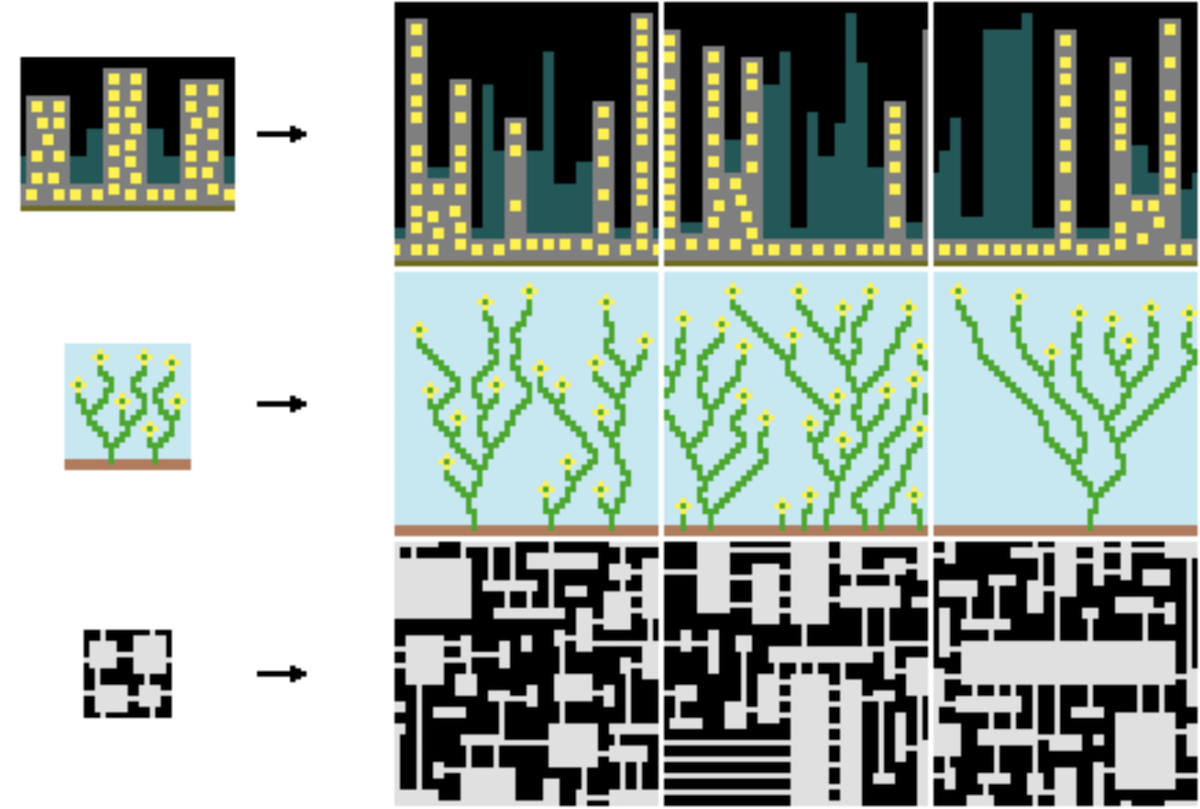
\includegraphics[scale=0.6]{obr/wfc-examples.png} % soubor + měřítko (scale)
  \caption{Příklad vzorů a výsledků \textit{WFC} \cite{waveClanek}} % popis obrázku
  \label{WFC_priklad} % definice odkazu na obrázek (pro \ref{})
\end{figure}

\subsection{GAN (Generative Adversarial Networks)}

\textit{Generativní adversariální sítě (GAN)} je metoda generování obsahu složená ze dvou komponent -- generátoru a diskriminátoru, které "bojují" v procesu učení. Generátor vytváří realistické výstupy napodobující reálná data. Diskriminátor se pak snaží rozlišit, zda jsou data reálná nebo vygenerovaná.

Princip metody \textit{GAN} právě spočívá v interakci mezi generátorem a diskriminátorem, díky které dochází k postupnému učení obou a tedy zlepšování kvality výsledných dat. Tento proces je řízen pomocí zpětné propagace, která umožňuje optimalizovat váhy v obou sítích. Toto vzájemné "soupeření" má za následek, že výsledná data systému \textit{GAN} vypadají realisticky i s menším množstvím vstupních reálných dat.

Mezi různé varianty \textit{GAN} patří například \textit{Deep Convolutional GAN (DCGAN}), který používá konvoluční vrstvy k lepšímu zachycení prostorových vzorců v datech. Tento přístup je možné využít při generování výškových map, nicméně má některá omezení, jako jsou problémy s velikostí a škálovatelností výstupů. Dále existuje, \textit{Spatial GAN (SGAN)} jedná se o vylepšenou variantu \textit{DCGAN}, která eliminuje plně propojené vrstvy a místo nich používá konvoluční vrstvy s \textit{krokem}, což umožňuje lépe zachovávat prostorové vztahy a zlepšuje efektivitu generování. \cite{GANclanek}



\section{Porovnání metod}

Popsal jsem několik možných přístupů generování herních map. V této části porovnám popsané metody generování map a zvolím vhodnou metodu, kterou implementuji v rámci tohoto výzkumného úkolu. 

Cílem je generovat herní mapu pro svět složený z políček nebo dlaždic pro strategickou hru, tedy výstup by měl připomínat přirozeně vypadající mapu světa. Tedy metody, které vytvářejí nesouvislé nebo lineárně rozdělené výsledky nejsou vhodné (nebudu se snažit generovat města, pouze krajinu). 

Zároveň, jelikož pro každou hru bude generována nová unikátní mapa, by bylo vhodné, aby generování probíhalo v rozumném čase, tedy metody s nízkou výpočetní náročností budou preferované.

Tabulka \vref{tabulka_metod} popisuje výhody a nevýhody jednotlivých metod generování.



\begin{sidewaystable}
\centering
\begin{tabular}{|l|l|l|}
\hline
\textbf{Metoda}                 & \textbf{Výhody}                                                                                                                     & \textbf{Nevýhody}                                                                                  \\ \hline
Space Partitioning              & \begin{tabular}[c]{@{}l@{}}Logická a hierarchická struktura\\ Snadné dosažení konzistentních výsledků\\ Vhodné pro vnitřní prostory\end{tabular}                                        & \begin{tabular}[c]{@{}l@{}}Výsledky můžou působit pravoúhle\\ Nevhodné pro organické mapy\end{tabular}                                      \\ \hline
Agent-Based generování          & \begin{tabular}[c]{@{}l@{}}Přirozené, nelineární výsledky\\ Velká variabilita výsledků\\ Snadné přizpůsobení chování agentů\end{tabular}                                                & \begin{tabular}[c]{@{}l@{}}Náročné ladění parametrů\\ Vysoká míra náhodnosti\\ Nepředvídatelné výsledky\end{tabular}                       \\ \hline
Grammar Algorithms              & \begin{tabular}[c]{@{}l@{}}Vysoká míra kontroly\\ Vhodné pro generování rozvržení úrovní\end{tabular}                                                                                   & \begin{tabular}[c]{@{}l@{}}Náročné na definování pravidel\\ Rychle narůstá složitost pravidel\\ Nevhodné pro přirozené terény\end{tabular} \\ \hline
Výškové mapy                    & \begin{tabular}[c]{@{}l@{}}Dobře reprezentují reálnou topografii\\ Plynulé přechody mezi výškovými úrovněmi\\ Snadná implementace \\ Snadná kombinace s dalšími technikami\end{tabular} & \begin{tabular}[c]{@{}l@{}}Náhodné generování vede k nereálným výsledkům\\ Nevhodné pro generování budov a interiérů\end{tabular}          \\ \hline
Fraktálové algoritmy            & \begin{tabular}[c]{@{}l@{}}Přirozeně vypadající krajina\\ Efektivní pro nekonečné terény\\ Relativně nenáročné na výkon\end{tabular}                                                   & \begin{tabular}[c]{@{}l@{}}Omezená kontrola\\ Výsledky mohou být homogenní\end{tabular}                                                    \\ \hline
Wave Function Collapse          & \begin{tabular}[c]{@{}l@{}}Konzistentní výsledky\\ Vhodné pro mapy s pravidelnými vzory\\ Snadné využití existujících vzorů\end{tabular}                                                                        & \begin{tabular}[c]{@{}l@{}}Výpočetně náročné\\ Složitý vstupní dataset\\ Může skončit ve stavu bez platného řešení\end{tabular}                                     \\ \hline
Generative Adversarial Networks & \begin{tabular}[c]{@{}l@{}}Realistické a variabilní výsledky\\ Adaptivní na různé typy prostředí\end{tabular}                                                                                                   & \begin{tabular}[c]{@{}l@{}}Velké množství trénovacích dat\\ Výpočetně náročné\\ Obtížně laditelné\end{tabular}                                                     \\ \hline
\end{tabular}
\caption{Porovnání metod generování prostředí}
\label{tabulka_metod}
\end{sidewaystable}

\newpage

Po porovnání metod generování map jsem se rozhodl využít \textit{metod výškových map}. Hlavním důvodem je, že tato metoda by měla být schopna generovat přirozeně vypadající krajinné útvary při poměrně nízké výpočetní náročnosti. Využití interpolace nebo gradientních metod umožní vytvářet plynulé přechody mezi různými typy terénu, což povede k realisticky vypadajícímu světu.

Mou další volbou by byla metoda \textit{Wave Function Collapse (WFC)} případně \textit{Generative Adversarial Networks (GAN)}, jelikož tyto metody mají potenciál vést k ještě realističtějším a více rozmanitým výsledkům. \textit{WFC} by zajistilo více vzorů v prostředí, zatímco \textit{GAN} by umožnilo generovat zcela nové mapy na základě trénovacích dat. Nicméně, obě tyto metody jsou výpočetně náročnější a vyžadují velká trénovací data, což je činí nevhodnými pro můj výzkumný úkol. Proto tyto metody ponechám jako případné možné rozšíření do diplomové práce.

\chapter{Implementace mapy}
\definecolor{darkgreen}{rgb}{0.0, 0.5, 0.0}   % Barva pro stringy
\definecolor{darkgray}{rgb}{0.3, 0.3, 0.3}    % Barva čísel řádků
\definecolor{codeblue}{rgb}{0.0, 0.0, 0.6}    % Barva pro klíčová slova
\definecolor{codegray}{rgb}{0.5, 0.5, 0.5}    % Neutrální šedá
\definecolor{commentgreen}{rgb}{0.0, 0.6, 0.0} % Barva pro komentáře

\lstdefinestyle{mystyle}{
    backgroundcolor=\color{white}, % pozadí kódu
    commentstyle=\color{commentgreen}\itshape,  % Celý komentář zeleně + kurzíva
    keywordstyle=\color{codeblue}\bfseries,     % Klíčová slova modře a tučně
    numberstyle=\tiny\color{darkgray},          % Čísla řádků šedě
    stringstyle=\color{darkgreen},              % Řetězce tmavě zeleně
    basicstyle=\ttfamily\footnotesize,          % Základní styl
    breakatwhitespace=false,
    breaklines=true,
    captionpos=b,
    keepspaces=true,
    numbers=left,
    numbersep=5pt,
    showspaces=false,
    showstringspaces=false,
    showtabs=false,
    tabsize=2,
    frame=single,
    extendedchars=true,
    morecomment=[l]#,
    literate=
      {á}{{\'a}}1 {č}{{\v{c}}}1 {ď}{{\v{d}}}1 {é}{{\'e}}1 {ě}{{\v{e}}}1 {í}{{\'i}}1
      {ň}{{\v{n}}}1 {ó}{{\'o}}1 {ř}{{\v{r}}}1 {š}{{\v{s}}}1 {ť}{{\v{t}}}1 {ú}{{\'u}}1
      {ů}{{\r{u}}}1 {ý}{{\'y}}1 {ž}{{\v{z}}}1
      {Á}{{\'A}}1 {Č}{{\v{C}}}1 {Ď}{{\v{D}}}1 {É}{{\'E}}1 {Ě}{{\v{E}}}1 {Í}{{\'I}}1
      {Ň}{{\v{N}}}1 {Ó}{{\'O}}1 {Ř}{{\v{R}}}1 {Š}{{\v{S}}}1 {Ť}{{\v{T}}}1 {Ú}{{\'U}}1
      {Ů}{{\r{U}}}1 {Ý}{{\'Y}}1 {Ž}{{\v{Z}}}1
}
\lstset{style=mystyle}

% Změna textu "Listing" na "Ukázka"
\renewcommand\lstlistingname{Ukázka}


\section{Generování herního pole}

Pro generování herního pole jsem zvolil metodu výškových map. Výšková mapa je dvourozměrná matice reálných čísel, kde každé číslo představuje výšku v daném bodě. Výškovou mapu následně převedu na konkrétní terénní typy, jako jsou voda, pláně, lesy a hory.

V této kapitole popíšu implementaci generování výškových map třemi způsoby:

\begin{itemize}
    \item Náhodná výšková mapa -- nejjednodušší metoda, která však vytváří nerealistický terén.
    \item Interpolace hrubé mřížky -- metoda, která vyhlazuje terén pomocí interpolace mezi body náhodné mřížky.
    \item Gradientní šum -- generování přirozeně vypadajícího terénu pomocí Perlinova šumu.
\end{itemize}

\section{Použité technologie}



\section{Implementované metody}

Výškové mapy jsem, jak už bylo zmíněno, implementoval třemi různými způsoby.

\subsection{Náhodná výšková mapa}

Tuto metodu jsem implementoval především proto, že je velmi jednoduchá a může sloužit jako základní benchmark pro srovnání s ostatními metodami. Výsledky této metody nejsou příliš dobré, protože nevytváří realistické terénní struktury. Výsledné struktury nejsou realistické ani praktické pro hraní.

Celá implementace spočívá v generování náhodných hodnot v a jejich uložení do dvourozměrného \textit{numpy} pole, které pak funkce vrací \ref{kod_nahodne_pole}.


\begin{lstlisting}[language=Python, caption=Kód generující pole pro náhodnou mapu, label=kod_nahodne_pole]
def nahodne_pole(rows, cols, min_value=0, max_value=1):
    return np.random.uniform(low=min_value, high=max_value, size=(rows, cols))

\end{lstlisting}


\subsection{Interpolovaná výšková mapa}

Lepšího výsledku lze dosáhnout interpolací náhodné mřížky. Tato metoda spočívá v tom, že vygeneruji menší náhodnou mřížku, tu rozmístím do větší a prázdné hodnoty získám interpolací hodnot z menší mřížky. Pro samotnou interpolaci využívám v kódu \ref{kod_interpolovane_pole} knihovnu \textit{scipy}. Funkce nakonec opět vrací matici čísel mezi nula a jedna.

\begin{lstlisting}[language=Python, caption=Kód generující iterpolovanou výškovou mapu, label=kod_interpolovane_pole]
def interpolovane_pole(big_rows, big_cols, small_rows, small_cols, min_value=0, max_value=1):
    # Vytvoření menší mřížky
    small_grid = nahodne_pole(small_rows, small_cols, min_value, max_value)
    # Indexy pro malou a velkou mřížku
    small_x = np.linspace(0, big_cols - 1, small_cols)
    small_y = np.linspace(0, big_rows - 1, small_rows)
    big_x = np.arange(big_cols)
    big_y = np.arange(big_rows)
    # Vytvoření seznamu souřadnic
    small_points = np.array([(x, y) for y in small_y for x in small_x])
    small_values = small_grid.flatten()
    big_points = np.array([(x, y) for y in big_y for x in big_x])
    # Doplnění hodnot seznamu interpolací
    big_list = griddata(small_points, small_values, big_points, method='cubic')
    # Převedení na mřížku
    big_grid = big_list.reshape(big_rows, big_cols)
    return big_grid

\end{lstlisting}

Interpolace vytvoří plynulejší terén bez ostrých přechodů mezi výškami, ale nevytváří přirozené detaily, jako jsou útesy nebo rozmanitější svahy.

\subsection{Gradientní šum}

Gradientní šum je komplikovanější metoda, která vytváří přirozenější struktury terénu než předchozí dvě metody. Konkrétně se inspiruji metodou \textbf{Perlinův šum}, který generuje plynulé změny hodnot v prostoru, čímž vytváří realistické krajiny s kopečky, údolími a horami.

Perlinův šum funguje na principu interpolace gradientních vektorů. Výsledkem je spojitá mapa hodnot, kde se výška plynule mění bez ostrých přechodů, ale vznikají přirozeně vypadající útvary. 

Tuto metodu jsem prvně implementoval pomocí knihovny \textit{noise} jako vzorový výsledek a následně jsem si také napsal vlastní implementaci.

\subsubsection{Vlastní implementace}

Mnou napsaná funkce generuje Perlinův šum v několika krocích:

\begin{enumerate}
    \item Vytvoření mřížky gradientových vektorů -- Každému bodu v hrubé mřížce (menší ze dvou mřížek, vytvořené podle zvolené hodnoty \textit{scale}) je přiřazen náhodný gradientový vektor. Tento vektor určuje, jak se bude hodnota šumu měnit v okolí daného bodu.
    \item Výpočet skalárních součinů -- Pro každý bod na jemné mřížce se vypočítá skalární součin mezi gradientními vektorem a vektorem k bodu, jehož hodnotu chceme určit.
    \item Použití funkce fade -- Hodnoty jsou vyhlazeny pomocí speciální funkce fade, která zajišťuje plynulý přechod mezi body mřížky a zabraňuje vzniku ostrých přechodů.
    \item Interpolace mezi sousedními hodnotami -- Hodnoty se interpolují mezi čtyřmi nejbližšími gradientními body, čímž vznikne plynulý přechod mezi oblastmi s různou výškou.
    \item Normalizace -- Nakonec se hodnoty normalizují aby výsledné hodnoty dobře vycházeli mezi hodnoty nula a jedna.
\end{enumerate}

Použitím různých měřítek (\textit{scale}) je možné ovlivnit rozmanitost a velikost útvarů vygenerované krajiny.

Výslednou matici hodnot, lze použít jako výškovou mapu pro tvorbu herního terénu. Výsledná mapa má plynulé přechody mezi různými výškami a vytváří přirozeně vypadající krajinu.

\subsection{Přiřazení typů terénu}

Po vygenerování výškové mapy je potřeba převést hodnoty na jednotlivé typy terénu, k tomu je použita funkce \texttt{cislo\_na\_policko} \ref{kod_cislo_na_policko}. 

\begin{lstlisting}[language=Python, caption=Převádějící výškovou mapu na konkrétní terény, label=kod_cislo_na_policko]
def cislo_na_policko(grid):
    mapa = np.empty_like(grid, dtype='str')
    for i in range(grid.shape[0]):  # Počet řádků
        for j in range(grid.shape[1]):  # Počet sloupců
            if grid[i][j] < 0.25:
                mapa[i][j] = "V"  # Voda
            elif grid[i][j] < 0.5:
                mapa[i][j] = "P"  # Pláně
            elif grid[i][j] < 0.75:
                mapa[i][j] = "L"  # Les
            else:
                mapa[i][j] = "H"  # Hory
    return mapa

\end{lstlisting}

Aktuální prahové hodnoty jsem zvolil experimentálně, ale mohou být upravovány po testování v simulaci, aby byl terén vyvážený a poskytoval vhodné herní prostředí.

\subsection{Vizualizace mapy}

Matici terénů vycházející z funkce \texttt{cislo\_na\_policko} pak zobrazuji pomocí \textit{matplotlib} pomocí funkce \texttt{zobraz\_mapu} \ref{kod_zobraz_mapu}.

\begin{lstlisting}[language=Python, caption=Kód generující pole pro náhodnou mapu, label=kod_zobraz_mapu]
def zobraz_mapu(mapa):
    """
    Barevně vykreslí terénní mapu.
    """
    # Definice barev pro jednotlivé typy terénu
    barvy = {
        "V": "#1f77b4",  # Modrá - Voda
        "P": "#58d162",  # Světle zelená - Pláně
        "L": "#0c3b10",  # Zelená - Les
        "H": "#4a4a48",  # Šedá - Hory
    }

    # Převedení mapy na numerickou matici s indexy
    text_to_index = {"V": 0, "P": 1, "L": 2, "H": 3}
    index_map = np.vectorize(text_to_index.get)(mapa)

    # Vytvoření barevné mapy
    cmap = ListedColormap(barvy.values())

    # Vykreslení mřížky
    plt.figure(figsize=(8, 8))
    plt.imshow(index_map, cmap=cmap, interpolation='nearest')

    plt.show()

\end{lstlisting}

Výstupem je čtyřbarevný graf složený ze čtvercových dlaždic.



\chapter{Návrh}
\section{Návrh strategické hry}

Zpracováno na základě: \cite{navrh_lenses} \cite{navrh_rules} \cite{navrh_level}.

V této kapitole rozeberu postup návrhu jednoduché strategické hry hrané na náhodně vygenerované mapě.

Návrh strategické hry vyžaduje systematický přístup k definování jejích klíčových prvků. Aby byla hra hratelná, vyvážená a pokud možno i zábavná, je zapotřebí systematicky rozebrat a promyslet návrh všech částí hry. 

Základní představa, se kterou jsem začínal před samotným systematickým návrhem, byla taková, že hra bude 2D tahová strategie s prvky správy surovin. Hráči budou ovládat a vylepšovat své jednotky, spravovat zdroje a budovat infrastrukturu, přičemž se budou snažit dosáhnout vítězství nad soupeřem. Herní svět je reprezentován dlaždicovou mapou, typ terénu na dlaždici ovlivňuje pohyb jednotek, možnosti výstavby a dostupnost zdrojů.

Pro návrh hry využívám metodologii z knihy \textit{The Art of Game Design: A Book of Lenses} od Jesseho Schella, která strukturuje herní design do několika klíčových kategorií:

\begin{itemize}
    \item Prostor -- Jak je herní svět uspořádán a jak se v něm hráči pohybují.
    \item Objekty, atributy a stavy -- Jaké herní entity existují, jaké mají vlastnosti a jaké stavy mohou při hře nastat.
    \item Akce hráče -- Jaké interakce může hráč provádět a jak ovlivňují hru.
    \item Pravidla hry -- Jaké jsou omezení a podmínky vítězství.
    \item Dovednost a náhoda -- Jaký je poměr mezi strategickým rozhodováním a prvky náhody.
\end{itemize}

Tento rámec poskytuje ucelený pohled na návrh hry a pomáhá zajistit, aby všechny prvky dohromady tvořily soudržný a dobře vyvážený celek.

Ve zbytku kapitoly rozeberu podrobněji právě tyto herní prvky a konkretizuji herní návrh.

%-------------------------------------------------------------------------
\subsection{Prostor}

Každá hra obsahuje nějaký herní prostor, ve kterém se celá hra odehrává. Ten obecně vymezuje herní lokace a určuje, jak jsou mezi sebou propojeny. Z pohledu herních mechanik považujeme prostor za matematickou konstrukci, tedy je potřeba odfiltrovat veškeré vizuální prvky a zaměřit se pouze na abstraktní uspořádání prostoru.

Kniha \textit{The Art of Game Design: A Book of Lenses} rozděluje herní prostory podle několika parametrů:

\begin{itemize}
    \item Diskrétnost vs. kontinuita -- Prostor může být buď diskrétní, nebo kontinuální. Diskrétní prostor je tvořen pevně stanovenými, oddělenými místy, kontinuální prostor umožňuje pohyb v plynulém, nekonečném rozsahu.
    \item Počet dimenzí -- Každý herní prostor má určitý počet dimenzí, které definují jeho rozsah a strukturu. Prostor může být jednorozměrný, dvourozměrný nebo dokonce třírozměrný, jak ukazuje například herní stůl na kulečník.
    \item Ohraničenost a propojení oblastí -- Prostor může být uzavřený, s pevně definovanými hranicemi, nebo otevřený, umožňující pohyb hráče nebo herních prvků mimo hranice. Rovněž je důležité zvážit, zda jsou jednotlivé části prostoru propojené, nebo zda jsou oddělené a nezávislé.
\end{itemize}

Příklad hry hrané na diskrétním dvoudimenzionálním poli je "piškvorky" (v rámci příkladu předpokládám herní plochu $3\times3$), kde herní plocha je rozdělena na devět oddělených políček. Herní deska je zobrazena jako souvislý prostor, ale z hlediska herních mechanik bereme v potaz pouze těchto devět specifických míst, která můžeme znázornit jako uzly v síti. Tedy dokud je jednoznačně rozeznatelné, do kterého políčka zapadá, jsou si mechanicky ekvivalentní, jak je naznačeno na obrázku \vref{sudoku}.

\begin{figure}
  \centering      % vycentrovat
  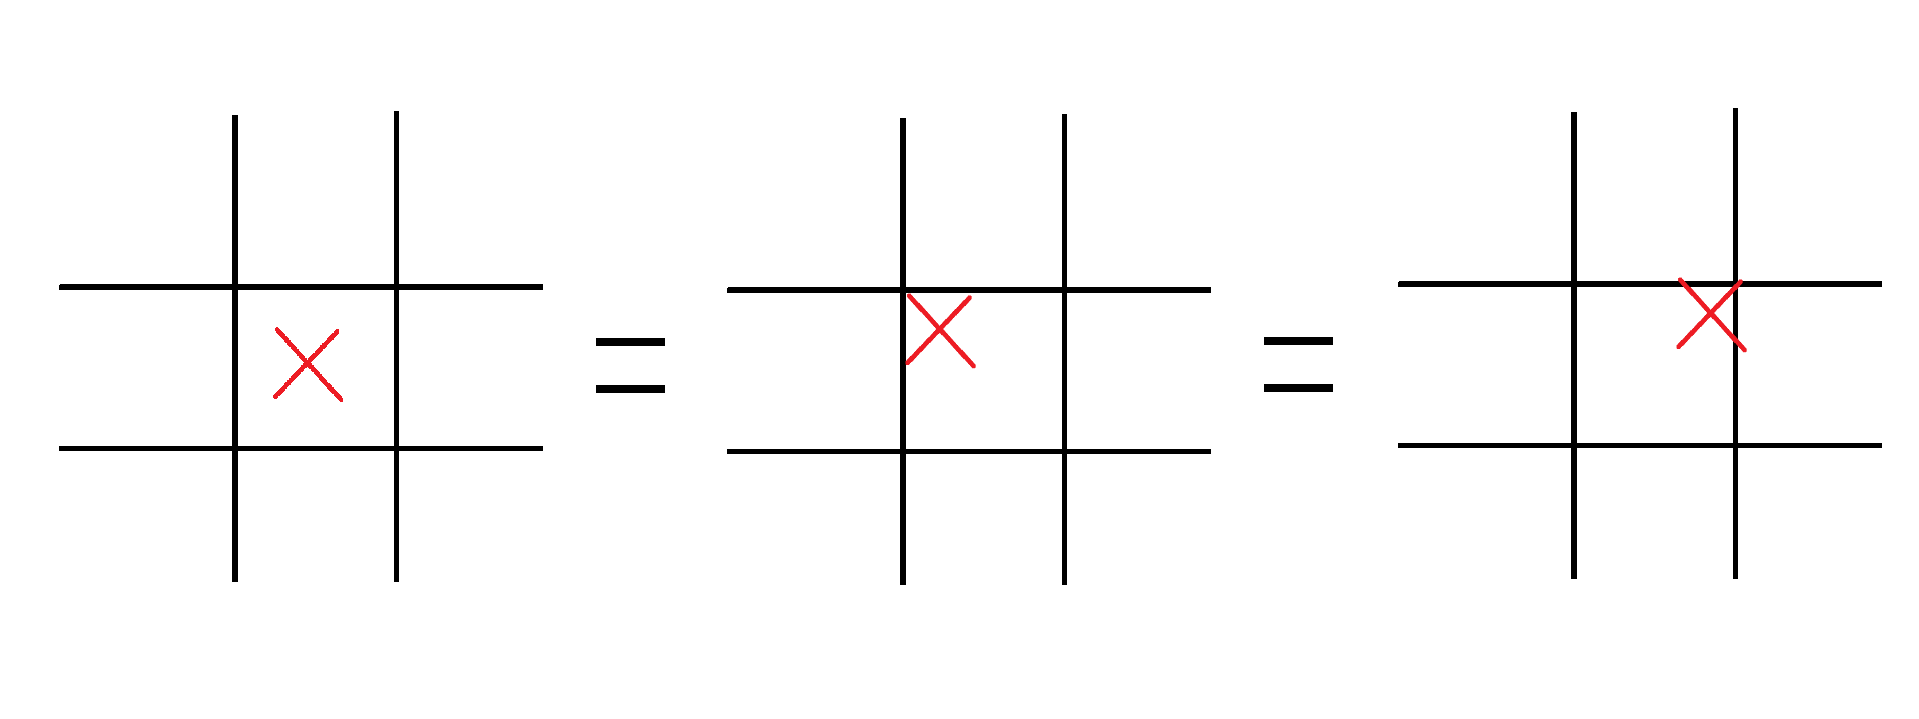
\includegraphics[scale=0.3]{obr/sudoku.png} % soubor + měřítko (scale)
  \caption{Ekvivalence různých značení sudoku.} % popis obrázku
  \label{sudoku} % definice odkazu na obrázek (pro \ref{})
\end{figure}

Hru monopoly pak můžeme definovat jako příklad jednodimenzionální hry. I když je herní deska vizuálně uspořádána do tvaru čtverce, když odstraníme grafické prvky, můžeme vidět, že hra umožňuje pohyb po jediné řadě políček, propojených v cyklické smyčce. V tomto případě se každé políčko na desce chová jako bod nulové dimenze, ačkoliv vizuálně vypadají některé čtverce odlišně, jejich funkce se neliší.

Herní prostor může také zahrnovat „prostory v prostorech“, což se často vyskytuje v počítačových hrách. Například může existovat venkovní prostor (kontinuální, dvourozměrný), ale hráč může narazit na ikony, které představují města nebo jeskyně. Tyto ikony přecházejí do zcela oddělených prostorů, které s venkovním prostorem nejsou přímo propojené, což je příkladem prostorového uspořádání, které je více založeno na mentálních modelech hráčů než na geografické realitě.

\subsubsection{Návrh herního prostoru}

Jak jsem již zmínil, navrhovaná hra bude 2D tahová strategie, tedy herní prostor bude dvoudimenzionální a diskrétní, složený ze čtvercových políček propojených po horizontální a vertikální ploše. To bude mít zásadní vliv na pohyb jednotek po mapě a tedy i veškerá strategická rozhodnutí hráčů.

Diskrétnost herního prostoru usnadňuje měření vzdáleností, po které se jednotky mohou po desce pohybovat, a také omezuje rozložení budov na jednu budovu na políčko. Stejně tak pro jednotky, což umožňuje strategické tahy, jako blokování pohybu jednotek nepřítele.

Ve hře nebudou žádné podprostory ani oblasti, které by hráči mohli navštívit jako separátní oblasti. Celý herní prostor tvoří jednotnou plochu bez vnitřních "meziprostorů" nebo propojení do nových sekcí. Všechny interakce probíhají na jednom herním poli, přičemž všechny herní mechaniky se soustředí na strategické využití této plochy.

Z hlediska návrhu a pozdější implementace tedy herní prostor uvažuji jako dvourozměrné diskrétní pole, kde každé "políčko" představuje bod s nulovou dimenzí. Tento pohled by měl zjednodušit návrh pravidel a interakcí mezi hráči a prostředím, což umožňuje efektivnější rozvoj herních taktik.

\subsubsection{Shrnutí prostoru}

Herní pole tedy pro účely návrhu uvažuji jako abstraktní dvoudimenzionální diskrétní prostor složený z políček propojených na ose $x$ a $y$. Hráči tedy budou moci pohybovat jednotkami pouze ve vertikálním či horizontálním směru, ne diagonálně. Prostor bude jasně vymezen hranicemi (konec vygenerované mapy) a všechny interakce mezi hráči budou probíhat na herní ploše. 

%-------------------------------------------------------------------------
\subsection{Objects, Attributes, and States (Objekty, atributy a stavy)}


V herním prostoru se pak nacházejí objekty se kterými hráči v průběhu celé hry manipulují nebo s nimi interagují pomocí jiných objektů. Může se jednat například o herní figurky, postavy, karty, nebo samotné herní prostředí. Objekty lze chápat jako „podstatná jména“ herních mechanik. 

Každý objekt má nějaké atributy, které popisují jeho vlastnosti. Atributy lze chápat jako "přídavná jména". Například auta v závodní hře mohou mít atributy jako \textit{maximální rychlost} a \textit{aktuální rychlost}. 

Každý herní objekt má \textbf{stav}, který určuje jeho vlastnosti a chování ve hře. Stav objektu se skládá z jeho atributů, což jsou jednotlivé charakteristiky objektu. Například figurka v šachu má atribut „mód pohybu“, který může nabývat stavů jako „volně se pohybující“, „v šachu“ a „matovaná“. V Monopoly má každý pozemek atribut „počet domů“, jehož stav se může měnit mezi 0 až 4 domy nebo hotelem.

Atributy mohou být statické nebo dynamické:

\begin{itemize} \item Statické atributy – Nemění se v průběhu hry. Například barva figurky v dámě nebo maximální rychlost auta.
\item Dynamické atributy – Mohou se měnit v závislosti na akcích hráčů či mechanikách hry. Například aktuální rychlost auta se mění podle řízení hráče, životy jednotky klesají při útoku. \end{itemize}

Každý herní objekt tak může mít kombinaci statických a dynamických atributů. Například v šachu má figurka statický atribut „barva“, ale dynamický atribut „pozice na šachovnici“, který se mění během hry.

Je důležité si uvědomit, že objekty ve hře často interagují mezi sebou. Například, jednotka může útočit na jinou jednotku, budova může produkovat suroviny, nebo terénní prvek může ovlivňovat pohyb jednotek. Tyto interakce by měly být navrženy tak, aby dávaly smysl a byly pro hráče srozumitelné.

Zásadní změny ve stavu herních objektů, ať už se jedná o změnu atributů nebo interakce s jinými objekty, je potřeba hráči nějakým způsobem indikovat. Vizuální reprezentace stavů objektů by měla být hráčům srozumitelná a intuitivní.

Stav objektu není nutně viditelný celý – některé atributy mohou být skryté nebo viditelné jen pro určité hráče.

Důležitou součástí herního návrhu tedy je rozhodnout, kdo má přístup k jakým informacím. Pro jednoduchost rozlišíme informace na \textit{veřejné} \textit{částečně skryté} nebo \textit{zcela skryté}. 

\begin{itemize}
    \item Veřejné informace -- Všechny atributy a jejich stavy jsou viditelné pro všechny hráče. Například v šachu oba hráči vidí všechna pole a figurky na hrací desce, takže jediným tajemstvím je přemýšlení soupeře.
    \item Částečně skryté informace -- Někteří hráči znají určitou informaci, ale jiní ne. Například ve hře poker někteří hráči viděli kartu, zatímco jiní ne.
    \item Zcela skryté informace -- Existují atributy, které zná pouze samotná hra. Například v počítačových hrách mohou být některé části světa před hráčem skryté, dokud je neodhalí.
\end{itemize}

Rozhodnutí o tom, kdo má přístup k jakým informacím, zásadně ovlivňuje herní strategii a atmosféru. Hry jako poker jsou postavené na utajení a odhadu soupeřových karet, zatímco v šachu mají hráči k dispozici informace o stavu celé herní plochy, a jedinou neznámou je strategie protivníka. Změna dostupnosti informací může radikálně proměnit hratelnost, například když se dříve skrytá informace náhle odhalí a změní dynamiku hry.

\subsubsection{Návrh herních objektů}

V této části se podle probraných principů pokusím nastínit jednotlivé objekty a definovat atributy těchto objektů.

Ve hře se nachází několik typů objektů, se kterými hráči mohou manipulovat nebo s nimi interagovat. Základním objektem ve hře jsou \textbf{políčka} ze kterých je složené herní pole a určují podmínky pro pohyb jednotek a stavbu budov. \textbf{Budovy}, produkují suroviny, případně poskytují další služby a plní jiné strategické funkce. Jako poslední jsou \textbf{jednotky} což jsou pohyblivé objekty ovládané hráčem, které hráč využívá k různým činnostem jako je boj, nebo těžba surovin. Každý z těchto objektů má své specifické atributy a stavy, které určují jejich vlastnosti a možnosti ve hře.

Co se informací týče nakonec jsem se rozhodl, že hra nebude mít skryté informace, tedy hráči od začátku uvidí celý herní prostor a pohyby protivníka.


\paragraph{Políčka}
Políčka představují základní stavební jednotku mapy, na níž se odehrává hra. Každé políčko má několik atributů, popisujících jeho vlastnosti a interakce s ostatními objekty. Tyto atributy jsou:
\begin{itemize}
    \item Statické:
    \begin{itemize}
        \item \textbf{Pozice na mapě} -- Souřadnice určující umístění políčka v herním prostoru.
        \item \textbf{Název} -- Název terénu.
        \item \textbf{Zpomalení} -- Určité typy terénů mohou snižovat pohybovou rychlost jednotek. 
        \item \textbf{Bonusová obrana} -- Některé terény mohou (např. Hory) mohou zvyšovat obranu jednotek na daném políčku.
        \item \textbf{Získatelné suroviny} -- Typ surovin které je možné na políčku získat.
    \end{itemize}
    \item Dynamické:
    \begin{itemize}
        \item \textbf{Obsazenost jednotka} -- Na políčku se může nacházet pouze jedna jednotka, tento atribut tedy bude bránit vstupu jiné jednotky na políčko.
    \item \textbf{Obsazenost budova} -- Na políčku může stát pouze jedna budova.
    \end{itemize}
%    \item \textbf{Možné zdroje} – některá políčka obsahují suroviny jako dřevo, kámen nebo jídlo. 
%    \item \textbf{Zpomalení} – některé terény zpomalují pohyb jednotek.
\end{itemize}

Terén není jen grafický prvek, ale významně ovlivňuje hru. Správná volba umístění jednotek může znamenat rozdíl mezi vítězstvím a porážkou – například jednotka stojící na horách má lepší obranu, zatímco husté lesy mohou zpomalit postup nepřátel. Navíc různé druhy terénu určují, jaké budovy lze postavit a jaké suroviny lze těžit.



\paragraph{Budovy}
Budovy jsou struktury, které hráči staví na mapě za účelem generování zdrojů nebo poskytování jiných výhod. Každá budova má následující atributy:
\begin{itemize}
    \item Statické:
    \begin{itemize}
        \item \textbf{Pozice na mapě} -- Pozice budovy na herní mapě.
        \item \textbf{Název} -- Označení budovy.
        \item \textbf{Vlastník} -- Určuje hráče, kterému budova patří. Změna vlastníků během hry nebude možná, poze zničení nepřátelských budov.
        \item \textbf{Typ terénu} -- Omezení, na kterých typech políček lze budovu postavit.
        \item \textbf{Produkce za kolo} – množství surovin, které budova generuje za kolo.
        \item \textbf{Životy max} -- Maximální počet životů budovy.
        \item \textbf{Obrana} -- O se zredukuje poškození způsobené útokem.
        \item \textbf{Cena} -- Množství surovin potřebných pro stavbu budovy.
        \item \textbf{Bonusová obrana} -- Budova může zvyšovat obranu jednotek nacházejících se na stejném políčku.
        \item \textbf{Speciální funkce} -- Budova může umožňovat provádění speciálních akcí jako generování nebo vylepšování jednotek.
    \end{itemize}
    \item Dynamické:
    \begin{itemize}
        \item \textbf{Životy} -- Aktuální počet životů budovy, pokud klesne na nulu budova je zničena.
    \end{itemize}
\end{itemize}
Budovy kromě generování surovin poskytují hráči jiné strategické možnosti jako vylepšování jednotek, zvyšování obrany vlastních jednotek nebo blokování postupu nepřítele.

\paragraph{Jednotky}
Jednotky jsou pohyblivé objekty na mapě, které hráči ovládají a skrze které primární interagují se s herními mechanismy. Každá jednotka má své atributy, které určují její vlastnosti a schopnosti:
\begin{itemize}
    \item Statické:
    \begin{itemize}
        \item \textbf{Název} -- Název typu jednotky.
        \item \textbf{Pozice na mapě} -- Kde na herním poli se jednotka nachází.
        \item \textbf{Vlastník} – hráč, kterému jednotka patří.
        \item \textbf{Cena} -- Množství surovin potřebné pro vytvoření jednotky.
        \item \textbf{Cena za kolo} -- Náklady na udržování jednotky. Množství surovin které jednotka spotřebuje každé kolo.
        \item \textbf{Životy max} -- Maximální počet životů jednotky.
         \item \textbf{Základní obrana} -- Základní obrana jednotky. Redukuje poškození způsobené nepřátelským útokem.
        \item \textbf{Útok} -- Síla útoku. Určuje o kolik se sníží životy nepřátelské jednotky při útoku. Poškození je redukované obranou. 
        \item \textbf{Dosah} -- Vzdálenost, na kterou může jednotka útočit.
        \item \textbf{Základní rychlost} – Maximální počet políček, která může jednotka urazit za kolo.
    \end{itemize}
    \item Dynamické:
    \begin{itemize}
        \item \textbf{Životy} -- Aktuální počet životů jednotky, pokud klesne na nulu jednotka zmizí.
        \item \textbf{Obrana} -- Funkční obrana jednotky, po modifikaci prostředím (Typem terénu nebo budovou.).
        \item \textbf{Rychlost} -- Skutečný počet políček přes který se jednotka může v daném tahu pohybovat, po modifikaci terénem.
        \item \textbf{Zaměstnaná} -- Indikuje, zda jednotka vykonala akci v tomto tahu.
        \item \textbf{V pohybu} -- Indikuje zda se jednotka v tahu pohybovala.
        \item \textbf{Zkušenosti} -- Jednotka může být vylepšena v konkrétní budově po dosažení určitého počtu zkušeností, které získává prováděním akcí odpovídajících jejímu typu (válečníci získávají zkušenosti bojem, pracovníci těžbou surovin nebo opravami budov).
    \end{itemize}
\end{itemize}

Jednotky představují hlavní způsob, jak hráč ovlivňuje dění na mapě. Každá jednotka má specifickou roli – některé slouží k boji, jiné k těžbě surovin nebo stavbě budov. Postupem času mohou získávat zkušenosti a vylepšovat své schopnosti, což přidává další vrstvu strategického rozhodování. Kromě toho jednotky také každé kolo spotřebovávají množství surovin, tedy hráč musí zvážit zda si může dovolit postavit velkou armádu slabých jednotek.


%-------------------------------------------------------------------------
\subsection{Actions (Akce hráče)}

Akce jsou jedním ze základních stavebních kamenů herní mechaniky. Lze je chápat jako "slovesa“ hry, jelikož definují, jak může hráč interagovat s herním světem. Rozdělujeme je do dvou hlavních kategorií: operační akce a výsledné (emergentní) akce.

\begin{itemize}
    \item \textbf{Operační akce} jsou základní činnosti, které může hráč přímo vykonat, například pohyb jednotky nebo útok.
    \item \textbf{Výsledné akce} vycházejí z kombinace operačních akcí. Tyto emergentní akce často nejsou přímo definovány pravidly, ale vznikají přirozeně během hry a přispívají k její hloubce.
\end{itemize}

\textbf{Operační akce} jsou základní mechanismy, které hráč využívá pro interakci s herními mechanismy. V některých hrách je množství těchto akcí omezené, což vede k menší variabilitě herního stylu, zatímco v jiných hrách mají hráči širokou škálu možností, což umožňuje kreativní přístupy. Například ve hře dáma má hráč k dispozici tři základní operační akce:
\begin{itemize}
    \item Posun kamene vpřed.
    \item Přeskok soupeřova kamene.
    \item Pohyb zpět v případě dosažení úrovně krále.
\end{itemize}

\textbf{Výsledné akce} vznikají kombinací operačních akcí a přispívají ke strategické hloubce hry. Zatímco operační akce jsou pevně dané pravidly, výsledné akce se objevují jako důsledek interakcí mezi hráčem, herním prostředím a protivníky.Ve hře dáma mohou být výslednými akcemi například:
\begin{itemize}
    \item Ochrana kamene -- umístění jiného kamene za něj, aby zabránil zajetí.
    \item Vynucení tahu soupeře -- postavení figurky tak, že soupeř musí provést nevýhodný tah.
    \item Obětování kamene -- nabídnutí figurky soupeři s cílem získat lepší pozici na hrací ploše.
\end{itemize}
Výsledné akce přidávají hře hloubku a umožňují emergentní chování hráče. Čím větší je poměr výsledných akcí vůči operačním akcím, tím více hra podporuje kreativitu hráče.

Zajímavé emergentní chování (výsledné akce) hry nevzniká náhodně, ale je to důsledek promyšleného návrhu herních mechanik. Existuje několik principů, jejichž aplikace může podpořit rozvoj interakce mezi herními prvky:

\begin{itemize}
    \item Rozšíření množiny operačních akcí -- Přidání nových základních akcí zvyšuje počet možných interakcí, čímž se rozšiřuje prostor pro emergentní chování.
    \item Univerzální využitelnost akcí -- Pokud lze jednu operační akci aplikovat na více objektů v herním prostředí, významně se tím zvyšuje počet možných výsledných akcí. Například zbraň nemusí sloužit výhradně k boji, ale může být využit k ničení překážek nebo aktivaci spínačů.
    \item Možnost dosažení cíle více způsoby – Hráči by měli mít možnost volit mezi různými strategiemi vedoucími k témuž cíli.
    \item Zvýšení počtu interagujících subjektů -- Počet možných výsledných akcí je úměrný množství prvků, které mohou vzájemně interagovat. Například v šachách vyplývá strategická hloubka hry nejen z možností pohybu jednotlivých figurek, ale i z jejich vzájemné spolupráce, blokování soupeřových tahů a vytváření kombinací.
    \item Vedlejší efekty herních akcí -- Pokud každá provedená akce kromě svého primárního účinku ovlivňuje i jiné aspekty hry, například mění dostupné možnosti pro soupeře či upravuje podmínky prostředí, dochází k tvorbě komplexnějších herních situací.
\end{itemize}

Akce hrají klíčovou roli v definování hratelnosti a interakce hráče s herním světem. I drobné úpravy v návrhu akcí mohou mít zásadní dopad na celkovou dynamiku hry, mohou buď poskytnout množství výsledných akcí, nebo naopak vést k repetitivní a předvídatelné hře. Z tohoto důvodu je třeba věnovat výběru a vyvážení herních akcí značnou pozornost.

\subsubsection{Návrh herních akcí}

V této části rozeberu obecné operační akce, které bude hráč moci ve hře provádět, a následně zmíním vzniklé výsledné akce.

V rámci tahového systému může hráč během svého tahu každou jednotkou provést pohyb a jednu další akci. Některé akce mohou proběhnout pouze pokud jsou splněny určité podmínky, například pozice jednotky v určité budově. Vzhledem k tahovému systému a interakci mezi jednotkami a terénem mohou vznikat nové strategie, které nelze vždy předvídat.

\paragraph{Operační akce} jsou základní činnosti, které může hráč vykonávat, primárně interakcí se svými jednotkami.
\begin{itemize}
    \item Pohyb -- Jednotka se pohne o počet polí odpovídající jejímu typu a terénu.
    \item Útok -- Jednotka zaútočí na nepřátelskou jednotku v dosahu, způsobí poškození (\textit{poškození = útok - obrana}) a pokud nepřítel přežije, provede protiútok.
    \item Těžba surovin -- Pracovní jednotka získá určité množství surovin na základě toho na jakém terénu těžba proběhne.
    \item Práce -- Pracovní jednotka v budově může získávat větší množství surovin, v budově která normálně generuje suroviny pasivně.
    \item Stavba budovy -- Budovatelská jednotka postaví novou budovu na vhodném políčku.
    \item Oprava budovy -- Pracovní nebo budovatelská jednotka obnoví část života poškozené budovy.
    \item Vylepšení jednotky -- Pokud jednotka splní požadavky (např. bojové zkušenosti, existenci potřebné budovy, ...), může být vylepšena na silnější variantu.
\end{itemize}

\paragraph{Výsledné akce} vznikají kombinací operačních akcí a strategického uvažování hráče.
\begin{itemize}
    \item Obrana klíčových bodů -- Hráč umístí jednotky tak, aby blokovaly přístup k důležitým budovám nebo oblastem.
    \item Napadání zásobování -- Cílený útok na pracovníky nebo budovy snižující zdroje nepřítele.
    \item Taktický ústup -- Ústup jednotek do bezpečnější oblasti, například k opravám nebo pod ochranu budov.
    \item Obklíčení -- Koordinovaný útok více jednotek k eliminaci klíčových nepřátel.
    \item Zdržovací taktika -- Hráč strategicky obětuje jednotky nebo využívá terén, aby zpomalil postup nepřítele.
    \item Ofenzivní opevnění -- Hráč staví budovy v nebo poblíž nepřátelské základy jako obranné pozice.
\end{itemize}


%-------------------------------------------------------------------------
\subsection{Rules (Pravidla hry)}

Pravidla určují, jak se hra hraje, jaké akce může hráč provádět a jaké jsou jeho cíle. Bez jasně definovaných pravidel není možné vytvořit funkční a férové herní prostředí. Pravidla nejenže vymezují hranice hratelnosti, ale také zásadně ovlivňují herní zážitek, určují tempo hry a strategické možnosti, které hra nabízí.

Špatně strukturovaná pravidla mohou vést k nevyváženosti, nechtěným exploatacím mechanik nebo dokonce ke ztrátě zábavnosti. Správně nastavená pravidla zároveň hráče motivují k objevování efektivních strategií a umožňují mu rozvíjet dovednosti potřebné k dosažení vítězství.


Pravidla jsou soubor omezení a možností, které definují, jak hráči interagují s herním světem. V každé hře existují různé typy pravidel, která ovlivňují hratelnost:

\begin{itemize}
    \item Akce hráčů -- Co mohou hráči během hry dělat?
    \item Stav hry -- Jak se hra mění v průběhu času?
    \item Cíle hry -- Kdy hra končí a kdo vyhrává?
\end{itemize}
Tato pravidla společně vytvářejí herní mechaniky, které určují dynamiku hry a poskytují hráčům výzvy k řešení.

David Parlett, britský herní teoretik, rozdělil pravidla do několika kategorií:

\begin{itemize}
    \item Operační pravidla -- Popisují základní akce hráčů, například „hráč se může pohnout o $n$ políček“.
    \item Základní pravidla -- Definují matematický model hry, určují, jak se hra vyvíjí na základě akcí hráčů.
    \item Chování hráčů -- Implicitní pravidla "fair play" a sportovního chování.
    \item Psaná pravidla -- Formálně dokumentovaná pravidla hry.
    \item Zákony -- Další pravidla, která mohou být zavedena například pro turnajovou hru.
    \item Oficiální pravidla -- Spojují psaná pravidla a zákony do jednoho uceleného souboru.
    \item Doporučená pravidla -- Tipy a strategie pro efektivní hraní.
    \item Domácí pravidla -- Úpravy pravidel hráči pro přizpůsobení hry jejich preferencím.
\end{itemize}

Herní pravidla mohou být ovlivněna herním režimem, který může do hry přidávat komplexitu přidáním nebo odebráním pravidel. Případně úpravou podmínek vítězství.

Nejdůležitějším pravidlem jsou cílové podmínky. Každá hra musí mít jasně definovaný cíl, který hráče motivuje a určuje, kdy hra končí. Dobrý cíl by měl splňovat:

\begin{itemize}
    \item Konkrétnost -- Je jasné, co musí hráči udělat.
    \item Dosažitelnost -- Hráči mají reálnou možnost dosáhnout cíle.
    \item Odměňující charakter -- Splnění cíle přináší uspokojení.
\end{itemize}

\subsubsection{Návrh pravidel}

V této části shrnu dosavadní návrh do konkrétních pravidel. Pravidla definují podmínky vítězství, možné akce hráčů a interakce mezi herními objekty.

Primárním cílem hry je poražení protivníka, což je dosaženo zničením všech jeho jednotek a budov. Hra tedy končí, když zůstane pouze jeden hráč.

Sekundární cíle si hráč stanovuje sám, ale zahrnují:

\begin{itemize}
    \item Efektivní správa ekonomiky -- těžba surovin a stavba podpůrných budov.
    \item Budování armády -- rekrutování a vylepšování jednotek.
    \item Dobývání strategických bodů -- kontrola území s cennými zdroji nebo taktickými výhodami.
\end{itemize}

\paragraph{Objekty} Hra obsahuje tři typy herních objektů:

\begin{itemize}
    \item Jednotky
    \begin{itemize}
        \item Bojové -- primárně slouží k útoku a obraně (např. válečník).
        \item Stavební -- mohou stavět nové budovy, opravovat poškozené budovy a těžit suroviny.
    \end{itemize}
    
    \item Budovy
    \begin{itemize}
        \item Ekonomické -- pasivně produkují zdroje (např. důl).
        \item Obranné -- poskytují ochranu a strategickou kontrolu území.
        \item Vývojové -- umožňují vylepšovat jednotky na vyšší úroveň.
    \end{itemize}
    
    \item Terén
    \begin{itemize}
        \item Ovlivňuje pohyb a bojové vlastnosti jednotek. (Např. hory zpomalují pohyb, lesy poskytují krytí, voda je nepřekročitelná.)
    \end{itemize}
    
\end{itemize}

\paragraph{Akce} V každém tahu může hráč provést s každou svou jednotkou jeden pohyb a jednu akci s tím, že některé akce vyžadují specifické podmínky, například vylepšení vyžadují určité budovy nebo sběr surovin má různý efekt podle terénu. Akce zahrnují:

\begin{itemize}
    \item Pohyb jednotek
    \begin{itemize}
        \item Každá jednotka se pohybuje pouze vertikálně a horizontálně, diagonální pohyb není možný.
        \item Terén ovlivňuje pohyb jednotek (např. hory snižují jejich pohybovou vzdálenost).
    \end{itemize}
    
    \item Útok
    \begin{itemize}
        \item Hráč vybere útočníka v dosahu.
        \item Útok je vyhodnocen podle atributů jednotek (útok vs. obrana).
        \item Pokud obránce přežije, provede protiútok.
    \end{itemize}
    
    \item Výstavba a interakce s objekty
    \begin{itemize}
        \item Stavební jednotky mohou budovat budovy na určitých místech.
        \item Pracovní jednotky mohou těžit suroviny, případně opravovat budovy
    \end{itemize}
\end{itemize}

\paragraph{Vynucování pravidel} Pravidla jsou automaticky vynucována herním systémem: Hráč může provádět pouze akce, které jsou v dané situaci povolené (např. jednotky nemohou cestovat přes políčka s vodou). Výsledky bojů jsou deterministické, hra tedy automaticky udělí způsobené poškození, případně zruší jednotku, pokud její životy klesnou na nulu. Hra automaticky končí, jakmile některý hráč přijde o všechny jednotky a budovy a tedy nemůže provést žádnou další akci.

%-------------------------------------------------------------------------
\subsection{Skill and Chance (Dovednost a náhoda)}
\begin{itemize}
    \item Jaký vliv má dovednost hráče na výsledek hry:
    \begin{itemize}
        \item Strategické plánování.
        \item Správné rozhodování a reakce na situace.
    \end{itemize}
    \item Jaký vliv má náhoda:
    \begin{itemize}
        \item Procedurálně generovaná mapa jako faktor variabilních podmínek.
    \end{itemize}
    \item Vyvážení mezi dovedností a náhodou.
\end{itemize}


%-------------------------------------------------------------------------
\subsection{Shrnutí}
\begin{itemize}
    \item Shrnutí hlavních bodů návrhu.
    \item Vztah návrhu k procedurálnímu generování map.
\end{itemize}


\chapter{Implementace základních mechanik}
\section{Implementace prototypu herních mechanik}

\subsection{Architektura a účel prototypu}

V tomto prototypu jsem implementoval základní herní mechaniky nezbytné pro provádění simulací a shromažďování dat, na jejichž základě budou v dalších fázích výzkumu rozšiřovány typy jednotek a budov a upravovány jejich statistiky. Architektura prototypu je založena na čtyřech klíčových třídách \ref{diagram_trid}, které zajišťují funkčnost herního cyklu a interakci mezi herními objekty:

\begin{itemize}
    \item \texttt{SpravceHry}: Centrální řídicí prvek, který spravuje průběh hry, střídání hráčů a implementuje základní umělou inteligenci. Zajišťuje koordinaci mezi ostatními třídami.
    \item \texttt{Hrac}: Reprezentuje jednotlivého hráče ve hře. Spravuje jeho ekonomiku (suroviny), vlastněné jednotky a budovy.
    \item \texttt{Jednotka}: Představuje herní jednotky s atributy jako útok, obrana, životy a pohyb.
    \item \texttt{Budova}: Reprezentuje hráčské budovy, které v prototypu primárně slouží k produkci surovin. Jejich implementace je v prototypu zjednodušená, spíše abstraktní.
\end{itemize}

Účelem tohoto prototypu je získat funkční základ pro simulace herních scénářů s různými konfiguracemi jednotek a budov. Získaná data poslouží k informovanému návrhu nových typů jednotek a budov a k úpravě jejich statistik pro dosažení vyvážené hratelnosti v plné verzi hry.

\begin{figure}
  \centering      % vycentrovat
  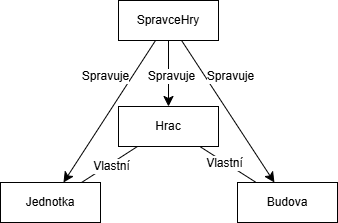
\includegraphics[scale=0.8]{obr/tridy.png} % soubor + měřítko (scale)
  \caption{Zjednodušený diagram tříd.} % popis obrázku
  \label{diagram_trid} % definice odkazu na obrázek (pro \ref{})
\end{figure}

\subsection{Třída \texttt{SpravceHry}}

Třída \texttt{SpravceHry} je hlavním řídicím prvkem celé hry. Zajišťuje koordinaci všech částí systému, spravuje průběh jednotlivých tahů a obsahuje také jednoduchou implementaci umělé inteligence ovládající hráče pro účely testování. Jedná se o centrální bod, který propojuje třídy \texttt{Hrac}, \texttt{Jednotka} a \texttt{Budova} a zabezpečuje jejich souhru v rámci herního cyklu.

Hlavní úlohy třídy zahrnují: 
\begin{itemize} 
    \item aktualizaci stavu hry v jednotlivých tazích, 
    \item správu střídání hráčů a ukončení hry při splnění podmínky vítězství, 
    \item rozhodování AI o pohybu a útocích jednotek. 
\end{itemize}

\paragraph{Aktualizace hry.}
Před začátkem hry je pomocí \texttt{inicializace\_hry} vytvořeno počáteční rozestavení hráčů včetně jejich základen a startovní ekonomiky (\texttt{startovni\_domek}).

Pomocí metody \texttt{aktualni\_hrac} se zjistí, který hráč je aktuálně na tahu. Střídání hráčů je zajištěno metodou \texttt{dalsi\_hrac}, která po odehrání všech hráčů zvyšuje číslo kola.

Při splnění podmínky vítězství (např. zničení základny) je hra ukončena metodou \texttt{konec}, která zaznamená výsledek a ukončí herní cyklus.

\paragraph{Provedení tahu.}
Metoda \texttt{proved\_tah} spravuje celý tah aktuálního hráče, včetně aktualizace surovin, vyhodnocení údržby jednotek a provedení akcí AI.

Metoda \texttt{kontrola\_bojeschopnosti} ověřuje, zda hráč po ztrátách ještě má bojeschopné jednotky.

\paragraph{Rozhodování AI.}  
Jednoduchá AI, implementovaná metodami \texttt{ai\_tah}, \texttt{ai\_pohyb\_a\_utok} a \texttt{stavba\_a\_verbovani\_ai}, vyhodnocuje akce jednotek hráče v daném tahu. Jednotky nejprve útočí na nejbližšího nepřítele v dosahu, pokud je k dispozici, nebo hledají nepřátelské jednotky v okolí jednoho kroku.Pokud ani tak nedosáhnou, posouvají se směrem k nepřátelské základně. Po pohybu jednotek, na základě aktuálního zisku surovin, AI rozhoduje o stavbě nových budov nebo verbování nových jednotek.

\paragraph{Verbování a Stavba}
Nové jednotky jsou vytvářeny metodou \texttt{verbovani}, která ověřuje podmínky a najde volné místo v okolí základny. 

Stavba budov probíhá obdobně metodou \texttt{stavba\_budovy}, pouze je zde na pevno daná pozice, jelikož umístění budov neberu v prototypu v potaz, pracuji 
s nimi jako s abstraktními.

\paragraph{Souboje}
Metoda \texttt{vyhodnot\_souboj} řeší útok jednotky na protivníka, včetně protiútoku a odstranění padlých jednotek. Pokud padne základna, hra je ukončena metodou \texttt{konec}.


\subsection{Třída \texttt{Hrac}}

Třída \texttt{Hrac} reprezentuje jednotlivého hráče ve hře. Uchovává jeho jméno, seznam jednotek a budov, dostupné suroviny. Hlavní odpovědností třídy je správa ekonomiky hráče, zejména manipulace se surovinami, zpracování údržby jednotek a vyhodnocení následků nedostatku zdrojů.

Hlavní úlohy třídy zahrnují: 
\begin{itemize} 
    \item správu zásob surovin a jejich změn, 
    \item evidenci vlastněných jednotek a budov, 
    \item zajištění výroby surovin budovami, 
    \item řešení údržby jednotek a následků nedostatku surovin. 
\end{itemize}

\paragraph{Práce se surovinami.}
Třída umožňuje přidávat nové suroviny pomocí metody \texttt{pridej\_suroviny} a odebírat suroviny pomocí \texttt{odecti\_suroviny}. Při odečítání je kontrolováno, zda má hráč dostatek požadovaných zdrojů.

\paragraph{Správa ekonomiky a údržby.}
Každé kolo může hráč získat nové suroviny produkované budovami prostřednictvím metody \texttt{zisk\_z\_budov}. Údržba jednotek je řešena metodou \texttt{zpracuj\_udrzbu}, která odečítá příslušné množství surovin. Pokud hráč nemá dostatek zdrojů, všechny jeho jednotky utrpí ztrátu životů.

\paragraph{Nedostatek jídla.}
Konkrétním případem správy ekonomiky je hladovění jednotek, implementované metodou \texttt{zpracuj\_nedostatek\_jidla}. Pokud hráč nemá dostatek jídla, jeho jednotky ztrácejí životy.


\subsection{Třída \texttt{Jednotka}}

Třída \texttt{Jednotka} reprezentuje jednu funkční jednotku ve hře. Její hlavní úlohou je definovat chování jednotky v rámci herního světa, včetně pohybu, boje a interakce s herním prostředím.

Hlavní úlohy třídy zahrnují:
\begin{itemize}
    \item uchovávání atributů jednotky (typ, pozice, statistiky, cena, vlastník),
    \item výpočet možných pohybů na základě rychlosti a terénu,
    \item realizaci pohybu na zvolenou cílovou pozici,
    \item vyhledávání nepřátelských jednotek v dosahu útoku,
    \item provádění útoku na nepřátelské jednotky a přijímání protiútoků,
    \item správu životů a mechanismus zániku jednotky.
\end{itemize}

\paragraph{Pohyb.}
Metoda \texttt{vypocet\_moznych\_pohybu} na základě aktuální pozice, rychlosti jednotky a typu terénu na herní mapě určuje všechny dosažitelné polohy. Při výpočtu zohledňuje překážky, jako je voda nebo přítomnost jiných jednotek. Metoda \texttt{proved\_pohyb} následně aktualizuje pozici jednotky, pokud je cílová pozice v seznamu možných pohybů.

\paragraph{Boj.}
Metoda \texttt{najdi\_cile\_v\_dosahu} prozkoumá okolí jednotky a vrátí seznam nepřátelských jednotek, které se nacházejí v jejím dosahu útoku. Samotný útok je realizován metodou \texttt{proved\_utok}, která sníží životy napadené jednotky na základě rozdílu mezi útočnou silou útočníka a obranou bránícího se, s případnými modifikátory terénu. Metoda \texttt{proved\_protiutok} umožňuje bránící se jednotce odpovědět na útok, pokud je útočník v jejím dosahu.

\subsection{Třída \texttt{Budova}}
Třída \texttt{Budova} obecně reprezentuje strukturu vlastněnou hráčem, která plní specifickou funkci v rámci hry. Může se jednat o budovy produkující suroviny, obranné stavby nebo jiné speciální budovy. Třída uchovává informace o typu budovy, její pozici na mapě, vlastníkovi, životech, obraně, produkci surovin a ceně za postavení.

Hlavní úlohy třídy zahrnují:
\begin{itemize}
    \item uchovávání atributů budovy (typ, pozice, vlastník, životy, obrana, produkce, cena),
    \item generování surovin.
\end{itemize}

\paragraph{Produkce surovin.}
Pokud je budova určena k produkci surovin, slovník \texttt{produkce} definuje typy surovin a jejich množství, které budova vyprodukuje za jedno herní kolo. Metoda \texttt{generuj\_suroviny} vrací tento slovník, čímž umožňuje hráči získávat zdroje.

\paragraph{Umístění.}
V tomto prototypu je pozice budovy pevně daná při jejím vytvoření a nelze ji měnit. Metoda pro stavbu budovy ve třídě \texttt{SpravceHry} zajišťuje její umístění na předdefinovanou pozici. V prototypu budovy neinteragují s pohybem jednotek ani mezi sebou, takže jejich přesné umístění nemá funkční dopad. 

\paragraph{Speciální funkce a blokování cesty.} Budovy mají v prototypu implementovanou pouze schopnost generovat suroviny. Jejich speciální schopnosti a schopnost blokovat cestu jsem se rozhodl implementovat až v rámci celé hry.

\chapter{Simulace}
\section{Simulace a testování}

V této kapitole popíšu průběh simulací zaměřených na získání dat pro vyvážení herních mechanik a určení optimálních parametrů jednotek, budov a herního pole. V simulacích budu využívat konkrétní scénáře a také metodu Monte Carlo pro získání robustních dat.

\subsection{Cíle simulací}

Hlavními cíli těchto simulací je:

\begin{itemize}
\item Systematicky testovat atributy jednotek, produkci budov a ceny herních prvků v různých scénářích.
\item Nalézt vyvážené nastavení herních parametrů, kde žádný prvek není výrazně dominantní nebo zbytečný.
\item Analyzovat charakteristiky generovaného herního pole v závislosti na jeho parametrech.
\end{itemize}

\subsection{Metriky pro sběr dat a analýzu}

Pro sběr dat a analýzu v těchto simulacích se zaměřím na následující metriky v rámci jednotlivých testovaných scénářů:

\begin{itemize}
    \item \textbf{Živé jednotky (kolo):} Počet živých jednotek daného typu patřících danému hráči na konci kola.
    \item \textbf{Způsobené poškození (kolo):} Celkové nominální poškození, které jednotky daného typu patřící danému hráči způsobily v daném kole.
    \item \textbf{Reálně způsobené poškození (kolo):} Celkové skutečné poškození, které jednotky daného typu patřící danému hráči způsobily v daném kole, s ohledem na obranu cíle a terénní modifikátory.
    \item \textbf{Utržené poškození (kolo):} Celkové poškození, které jednotky daného typu patřící danému hráči utrpěly v daném kole.
    \item \textbf{Počet útoků (kolo):} Celkový počet útoků provedených jednotkami daného typu patřícími danému hráči v daném kole. Pomáhá pochopit aktivitu jednotek v boji.
    \item \textbf{Počet protiútoků (kolo):} Celkový počet protiútoků provedených jednotkami daného typu patřícími danému hráči v daném kole. Zaznamenává dodatečnou bojovou aktivitu.
    \item \textbf{Vítězství:} Který hráč vyhrál simulaci
    \item \textbf{Míra přežití jednotek (výsledek simulace):} Procento jednotek daného typu, které přežily celý střet.
    \item \textbf{Poškození (výsledek simulace):} Celkové poškození způsobené jednotkou daného typu během celého střetu.
    \item \textbf{Zranění (výsledek simulace):} Celkové poškození, které jednotka daného typu utrpěla během celého střetu.
    \item \textbf{Poměr ztrát (výsledek simulace):} Poměr mezi celkovým způsobeným poškozením a celkovým utrženým poškozením pro každou stranu v daném scénáři, nebo poměr počtu ztracených jednotek.
    \item \textbf{Počet kol (výsledek simulace):} Celkový počet kol, po kterých hra skončila.
    \item \textbf{Ekonomická efektivita (výsledek simulace):} Poměr mezi investovanými surovinami (náklady na jednotky) a dosaženými výsledky (např. celkové způsobené poškození).
\end{itemize}

\section{Teorie simulace}

Při provádění simulací budu využívat přístup podobný Monte Carlo metodě. Tato metoda spočívá v opakovaném náhodném vzorkování a simulaci s cílem získat statisticky robustní odhady chování komplexních systémů. 

V kontextu této práce to znamená, že jednotlivé testovací scénáře a celkové herní simulace budou spouštěny mnohokrát s potenciálně mírně odlišnými počátečními podmínkami (zejména v pozdějších fázích s náhodně generovanými mapami a prvkem náhody v rozhodování AI), abych získal průměrné výsledky a posoudil stabilitu a vyváženost herních mechanismů.

\subsection{Fáze 1: Testování vyváženosti jednotek a ekonomických parametrů v izolovaných scénářích}

V této fázi se zaměřím na testování jednotlivých typů jednotek proti sobě v kontrolovaných bojových situacích a zároveň budu zkoumat vliv cen jednotek a produkce surovin na jejich efektivitu.

\begin{itemize}
    \item \textbf{Scénáře 1v1:} Budu simulovat souboje mezi dvěma jednotkami různých typů (např. bojovník vs. lučištník) se stejnou nebo podobnou cenou.
    \item \textbf{Scénáře "armáda proti armádě":} Budu simulovat střety mezi menšími skupinami jednotek (např. 3 bojovníci vs. 2 lučištníci a 1 bojovník) se srovnatelnou celkovou cenou.
\end{itemize}

V rámci těchto scénářů mohu simulovat, jak rychlost získávání surovin ovlivňuje schopnost hráčů nasazovat jednotky v různých typech střetů.
Budu analyzovat, jak cena jednotky ovlivňuje její výkonnost v boji a její ekonomickou návratnost v kontextu verbování.

Na základě výsledků budu upravovat atributy a ceny jednotek a produkci budov a testovat upravené verze v nových scénářích.

\subsection{Fáze 2: Testování náhodného herního pole}

V této fázi se zaměřím na analýzu charakteristik generovaného herního pole v závislosti na parametrech generování mapy. Budu testovat různé kombinace parametrů, jako je velikost mapy, škálování Perlinova šumu a prahové hodnoty pro definici jednotlivých typů terénu. Pro každé nastavení budu provádět opakované generování map a sbírat následující statistiky:

\begin{itemize}
\item \textbf{Existence cesty mezi základnami:} Pro každou vygenerovanou mapu zjistím, zda existuje alespoň jedna průchodná cesta mezi počátečními pozicemi základen (předpokládám pevně dané startovní pozice pro účely tohoto testování).
\item \textbf{Délka nejkratší cesty mezi základnami:} Pokud cesta existuje, vypočítám délku nejkratší cesty (například pomocí algoritmu A* nebo Dijkstrova algoritmu s ohodnocením políček podle typu terénu).
\item \textbf{Existence "snadné" cesty (bez hor):} Zjistím, jak často existuje cesta mezi základnami, která neprochází přes horský terén ('H').
\item \textbf{Poměr zastoupení jednotlivých typů terénu:} Pro každou vygenerovanou mapu spočítám procentuální zastoupení jednotlivých typů terénu (voda 'V', pláně 'P', les 'L', hory 'H').
\end{itemize}

Cílem této fáze je identifikovat parametry generování map, které vedou k herním polím s vhodnými charakteristikami z hlediska průchodnosti, strategické hloubky (dané rozložením terénu) a potenciálu pro interakci mezi hráči.

\subsection{Fáze 3: Testování v celkových herních simulacích na náhodně generovaných mapách}

V této fázi se vrátím k simulacím celých her na náhodně generovaných mapách s jednoduchou AI, s již předběžně vyladěnými parametry jednotek a produkce budov z Fáze 1 a s nastavením generování map z Fáze 2, které se ukázalo jako nejvhodnější.

\begin{itemize}
\item \textbf{Sledování celkové dynamiky hry:} Budu sledovat délku her, frekvenci interakcí mezi hráči a celkový průběh hry.
\item \textbf{Sbírání dat pro finální doladění:} Budu shromažďovat data o využití jednotek a budov, výsledcích střetů a ekonomickém vývoji hráčů v reálných herních podmínkách pro případné další úpravy parametrů.
\end{itemize}

\section{Simulace}
V plné hře bude možné koupit pouze jednotky Pracovník a Bojovník, které pak hráč s použitím budov bude moci vylepšovat. Tento mechanismus není v prototypu implementován takže se v rámci simulace budu muset spokojit s odlišnou cenou jednotek na různé úrovni.

% TODO: Obrázek evoluce jednotek

Typy jednotek a jejich arbitrárně vybrané atributy jsou vidět v tabulce \ref{tab:atributy_jednotek_otocena}. S těmito hodnotami začneme testovat jednotky proti sobě a upravovat jejich vlastnosti dokud nebudou podobně hodnotné jednotky vykazovat podobnou sílu.

\newpage

\begin{sidewaystable}[h!]
\centering
\begin{tabular}{|l|*{9}{c|}}
\hline
\textbf{Atribut} & \textbf{Bojovník} & \textbf{Válečník} & \textbf{Rytíř} & \textbf{Berserkr} & \textbf{Lučištník} & \textbf{Ostrostřelec} & \textbf{Lovec} & \textbf{Základna} \\
\hline
Rychlost & 3 & 3 & 2 & 4 & 3 & 2 & 5 & 0 \\
\hline
Dosah & 1 & 1 & 1 & 1 & 4 & 6 & 3 & 0 \\
\hline
Útok & 5 & 8 & 10 & 12 & 7 & 10 & 7 & 0 \\
\hline
Obrana & 3 & 5 & 7 & 2 & 2 & 1 & 2 & 0 \\
\hline
Životy & 10 & 15 & 30 & 20 & 10 & 10 & 14 & 50 \\
\hline
Cena (jidlo) & 10 & 60 & 120 & 70 & 15 & 80 & 60 & 0 \\
\hline
Cena (dřevo) & 2 & 30 & 50 & 40 & 15 & 60 & 40 & 0\\
\hline
Cena (kámen) & 0 & 0 & 30 & 0 & 0 & 40 & 0 & 0 \\
\hline
Cena/kolo (jidlo) & 2 & 3 & 4 & 4 & 2 & 4 & 3 & 0 \\
\hline
Cena/kolo (dřevo) & 0 & 0 & 0 & 0 & 1 & 2 & 1 & 0 \\
\hline
Cena/kolo (kámen) & 0 & 0 & 1 & 0 & 0 & 0 & 0 & 0 \\
\hline
\end{tabular}
\caption{Atributy jednotek pro začátek simulace}
\label{tab:atributy_jednotek_otocena}
\end{sidewaystable}

\newpage


\subsection{Fáze 1: Základní vyvážení (1v1):}

V této fázi se zaměřím na testování jednotlivých typů jednotek proti sobě v kontrolovaných bojových situacích. 

Počáteční podmínky jsou známé a stálé a absence náhody v rozhodování AI to znamená, že výsledek každé jednotlivé simulace daného scénáře je vždy stejné, bude počet opakování snížen na deset. To slouží k ověření konzistence a zachycení případných anomálií, aniž by docházelo ke zbytečným výpočetním nárokům.

\paragraph{Mapy:}
\begin{itemize}
    \item \textbf{Rovná linie}
        \begin{itemize}
            \item \textbf{Mapa:} Linie (15 polí typu 'P' - pláně).
            \item \textbf{Umístění jednotek:} Jednotky budou začínat na opačných stranách linie (0, 0) a (14, 0).
            \item \textbf{Očekávané efekty a cíle:} Tento scénář testuje přímí souboj dvou jednotek bez možnosti manévrování nebo využití terénu. Cílem je porovnat jednotky v přímém boji bez manévrování.
        \end{itemize}
    \item \textbf{Rovina (velká otevřená plocha)}
        \begin{itemize}
            \item \textbf{Mapa:} Rovina (velká obdélníková mapa, 15x15 polí typu 'P' - pláně).
            \item \textbf{Umístění jednotek:} Jednotky budou začínat v opačných rozích (0, 0) a (14, 14).
            \item \textbf{Očekávané efekty a cíle:} Zvětšení celkové plochy poskytne prostor pro manévrování a ustupování.  Bude zde potřeba pohyb ve více směrech ne jen dopředu, což může mít vliv na efektivitu jednotek v boji. Cílem je zjisti zda otevřený prostor ovlivní výsledky.
        \end{itemize}
    \item \textbf{Pohoří (s horami uprostřed)}
        \begin{itemize}
            \item \textbf{Mapa:} Pohoří (obdélníková mapa, 15x15 s horami 'H' rozdělujícími mapu napůl oblepenými lesy).
            \item \textbf{Umístění jednotek:} Jednotky budou začínat v opačných rozích (0, 0) a (14, 14).
            \item \textbf{Očekávané efekty a cíle:} Horský terén ('H') modifikuje obranu jednotek stojících na něm (+2 obrana), zároveň ale také zásadně zpomaluje pohyb. To může mít zásadní dopad na souboj. Cílem je kvantifikovat, jak moc terén ovlivňuje balanc souboje.
        \end{itemize}
\end{itemize}

\subsubsection{Válečník vs. Lučištník}

Tento duel představuje souboj dvou základních archetypů jednotek po prvním vylepšení, z nichž se dále odvíjí celá evoluční větev jednotek. Cílem je posoudit, jak se odlišné atributy Válečníka (vyšší obrana a životy, kontaktní boj) a Lučištníka (dálkový útok, mobilita a schopnost ústupu) projeví na různých typech terénu. Očekáváme, že na rovinatých mapách s dostatkem prostoru bude Lučištník moci efektivněji využít manévrování, zatímco na lineární mapě bude souboj přímější a Válečník by mohl mít výhodu. Horský terén by pak měl výrazně zvýhodnit Lučištníka díky svým obranným bonusům a vlivu na pohyb.


\paragraph{Rovná linie}~ \newline

\textbf{Počáteční atributy:}
\begin{itemize}
\item \textbf{Jednotka A (Válečník):} \\ Útok:~8, Obrana:~5, Životy:~15, Rychlost:~3, Dosah:~1, \\ Cena (jídlo/dřevo/kámen):~60/30/0
\item \textbf{Jednotka B (Lučištník):} \\ Útok:~7, Obrana:~2, Životy:~10, Rychlost:~3, Dosah:~4, \\ Cena (jídlo/dřevo/kámen):~15/15/0
\end{itemize}

\textbf{Výsledky simulace (agregace 10 simulací):}
\begin{itemize}
\item \textbf{Poměr vítězství:} Válečník: 100\% simulací, Lučištník: 0\% simulací.
\item \textbf{Průměrný počet kol:} 4 kola
\item \textbf{Průměrné způsobené poškození za kolo (Válečník):} 3.00
\item \textbf{Průměrné způsobené poškození za kolo (Lučištník):} 1.50
\item \textbf{Průměrné utržené poškození za kolo (Válečník):} 1.50
\item \textbf{Průměrné utržené poškození za kolo (Lučištník):} 3.00
\item \textbf{Průměrný počet útoků za kolo (Válečník):} 0.50
\item \textbf{Průměrný počet protiútoků za kolo (Válečník):} 0.00
\item \textbf{Průměrný počet útoků za kolo (Lučištník):} 0.50
\item \textbf{Průměrný počet protiútoků za kolo (Lučištník):} 0.25
\item \textbf{Průměrná míra přežití (Válečník):} 100.00\%
\item \textbf{Průměrná míra přežití (Lučištník):} 0.00\%
\end{itemize}

\begin{figure}
  \centering      % vycentrovat
  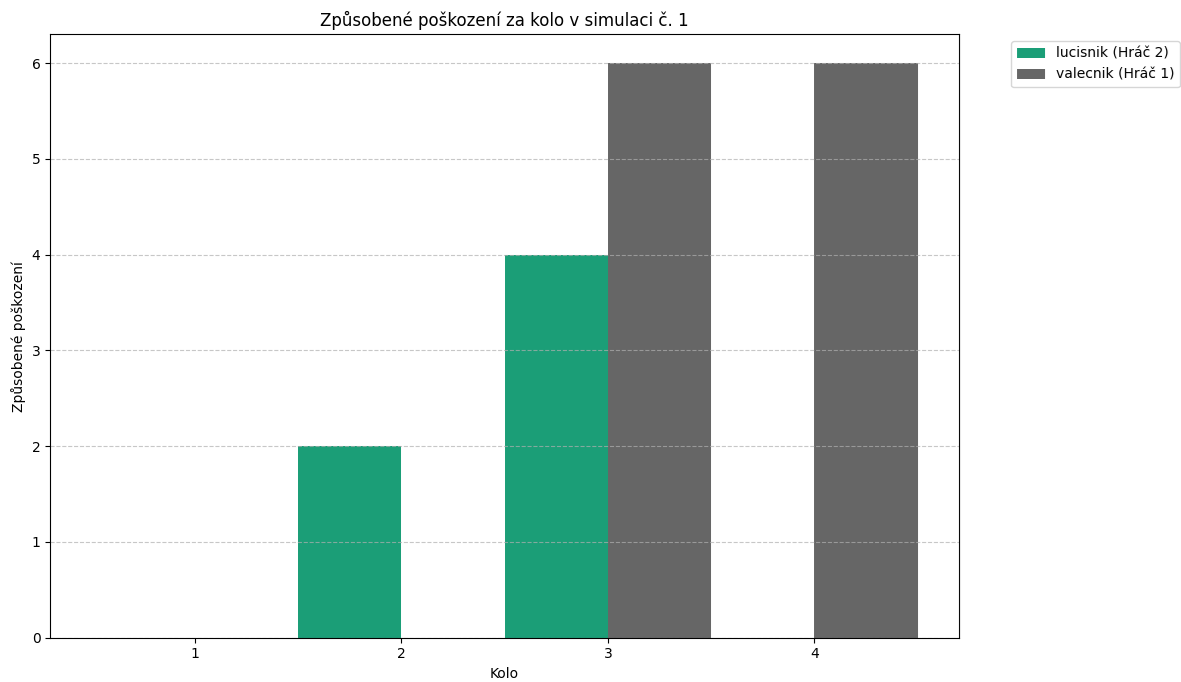
\includegraphics[scale=0.5]{obr/graf_valVSluc_linie_damage.png} % soubor + měřítko (scale)
  \caption{Graf poškození které jednotky způsobili v každém kole simulace} % popis obrázku
  \label{graf_valVSluc_linie_damage} % definice odkazu na obrázek (pro \ref{})
\end{figure}

\begin{figure}
  \centering      % vycentrovat
  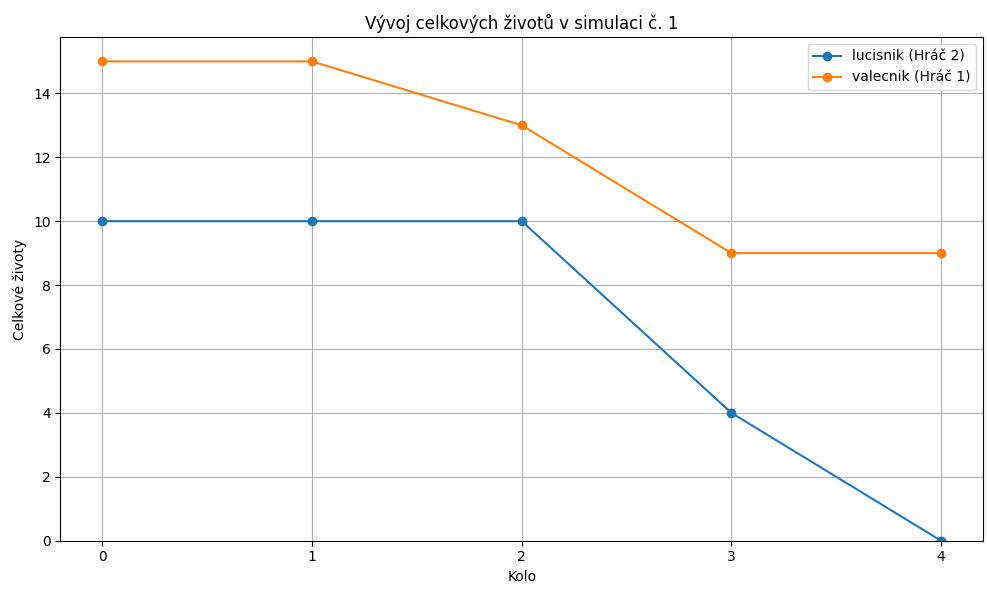
\includegraphics[scale=0.5]{obr/graf_valVSluc_linie_HP.png} % soubor + měřítko (scale)
  \caption{Graf životů jednotek v průběhu simulace} % popis obrázku
  \label{graf_valVSluc_linie_HP} % definice odkazu na obrázek (pro \ref{})
\end{figure}

\textbf{Analýza dat a interpretace:}

Na mapě Rovná linie, kde dochází k přímému střetu bez možnosti manévrování, se jasně ukázala \textbf{dominance Válečníka}, který zvítězil během průměrně 4 kol. Válečník způsobil průměrně 3.00 poškození za kolo a útočil s frekvencí 0.50 útoků za kolo, zatímco Lučištník způsobil 1.50 poškození za kolo se stejnou frekvencí útoků 0.50 za kolo. Lučištník navíc zaznamenal průměrně 0.25 protiútoků za kolo, což znamená, že poškození způsobil vícekrát než válečník. Zároveň je z obrázku \ref{graf_valVSluc_linie_HP} vidět, že válečník na konci neztratil ani polovinu svých životů.

Z toho je vidět, že útočná síla lučištníka je oproti obraně válečníka příliš malá, ačkoliv provedl více útoků, způsobil výrazně menší poškození. Tedy buď je potřeba snížit obranu válečníka, nebo zvýšit útok lučištníka.

\textbf{Navrhované úpravy atributů a zdůvodnění:}

Pro dosažení lepší vyváženosti v přímém souboji a zvýšení relevantnosti Lučištníka zkusím tyto úpravy a uvidím jak vyplyne souboj:

\begin{itemize}
    \item \textbf{Lučištník:}
    \begin{itemize}
        \item \textbf{Útok:} Zvýšení ze 7 na \textbf{8}.
        \item \textbf{Obrana:} Zvýšení z 2 na \textbf{3}.
        \item \textbf{Zdůvodnění:} Zvýšením útoku se Lučištník vyrovná Válečníkovi v základním poškození, což by mělo vést k efektivnějšímu snižování Válečníkových životů. Mírné navýšení obrany pak Lučištníkovi poskytne drobnou, ale potenciálně klíčovou výhodu pro přežití jednoho dalšího kola, což mu umožní způsobit více celkového poškození.
    \end{itemize}
    \item \textbf{Válečník:}
    \begin{itemize}
        \item \textbf{Obrana:} Snížení z 5 na \textbf{4}.
        \item \textbf{Zdůvodnění:} Snížení obrany Válečníka zvýší poškození, které obdrží od Lučištníka. To by mělo vést k rychlejšímu průběhu souboje z pohledu Válečníka a celkově vyrovnanějšímu střetu.
    \end{itemize}
\end{itemize}

\paragraph{Ověření úprav na mapě Rovná linie:}~ \newline

Po provedení navržených úprav jsem zopakoval simulaci na Linii.

\textbf{Nové výsledky simulace:}
\begin{itemize}
\item \textbf{Poměr vítězství:} Válečník: 100\% simulací, Lučištník: 0\% simulací.
\item \textbf{Průměrný počet kol:} 4 kola.
\item \textbf{Průměrné způsobené poškození za kolo (Válečník):} 2.50
\item \textbf{Průměrné způsobené poškození za kolo (Lučištník):} 3.00
\item \textbf{Průměrná míra přežití (Válečník):} 100.00\%
\item \textbf{Průměrná míra přežití (Lučištník):} 0.00\%
\end{itemize}

\begin{figure}
  \centering      % vycentrovat
  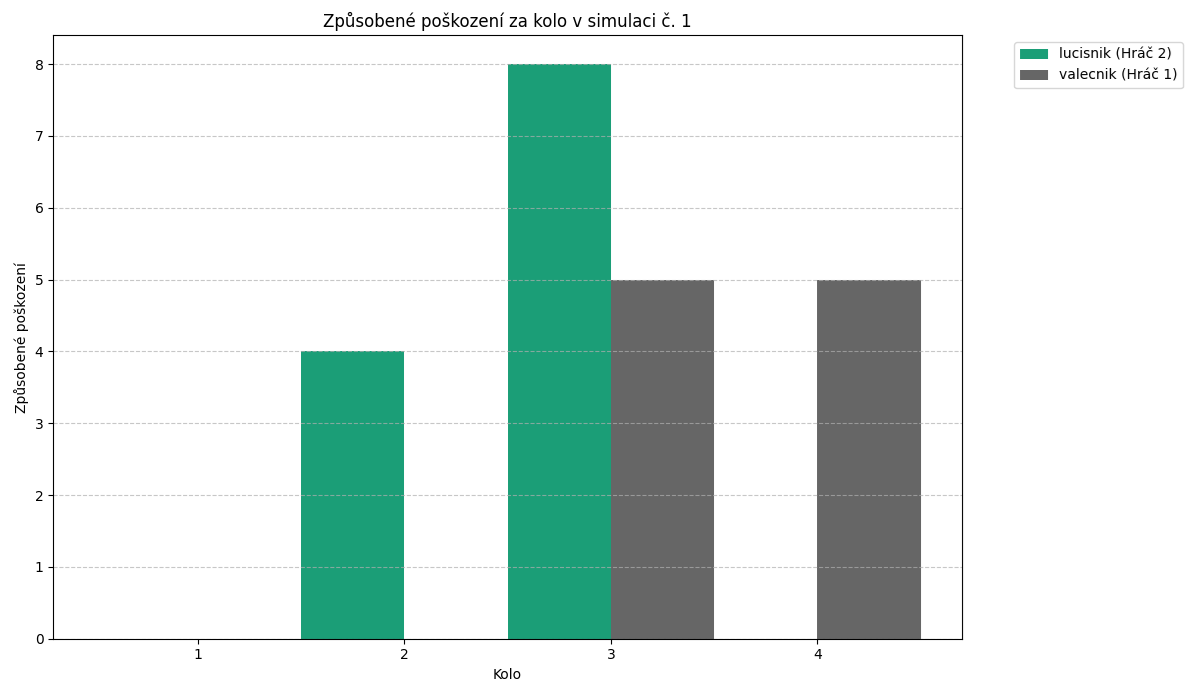
\includegraphics[scale=0.5]{obr/graf_valVSluc_linie_damage2.png} % soubor + měřítko (scale)
  \caption{Graf poškození které jednotky způsobili v každém kole simulace} % popis obrázku
  \label{graf_valVSluc_linie_damage2} % definice odkazu na obrázek (pro \ref{})
\end{figure}

\begin{figure}
  \centering      % vycentrovat
  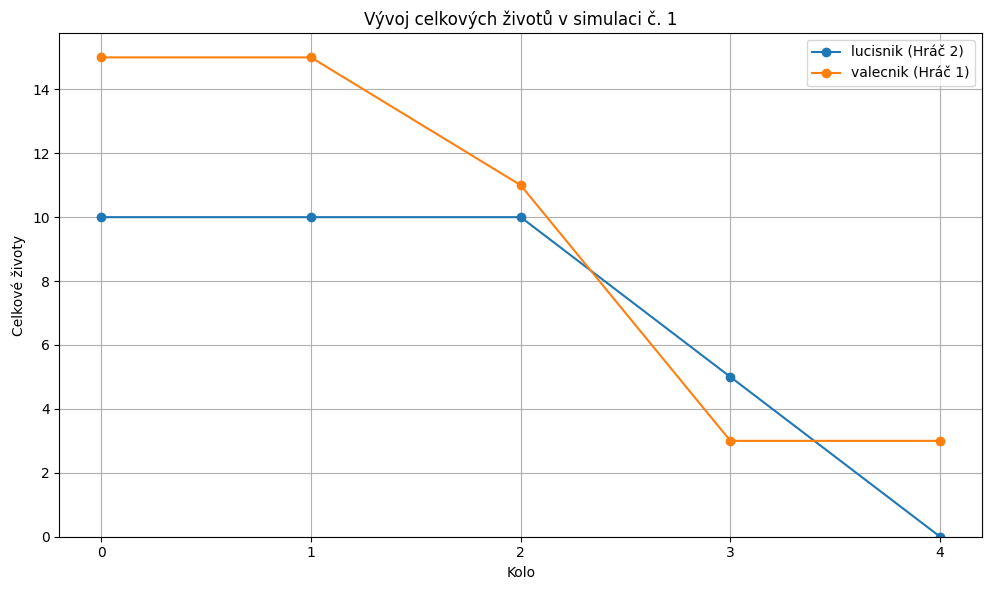
\includegraphics[scale=0.5]{obr/graf_valVSluc_linie_HP2.png} % soubor + měřítko (scale)
  \caption{Graf životů jednotek v průběhu simulace} % popis obrázku
  \label{graf_valVSluc_linie_HP2} % definice odkazu na obrázek (pro \ref{})
\end{figure}

Ačkoliv Válečník stále vyhrává všechny simulace, data ukazují jasné známky zlepšení vyvážení. Lučištník nyní průměrně způsobuje více poškození za kolo (3.00) než Válečník (2.50), což je zásadní obrat oproti předchozím simulacím.

Z grafu \ref{graf_valVSluc_linie_HP2} průběhu životů je patrné, že souboj je nyní mnohem vyrovnanější. Válečník končí simulace s pouze čtyřmi životy, což je výrazně nižší hodnota než před úpravami. Graf poškození \ref{graf_valVSluc_linie_damage2} navíc potvrdil, že ve druhém kole Lučištník skutečně způsobil větší poškození než Válečník, což demonstruje jeho zvýšenou útočnou efektivitu v klíčových momentech boje.

Tyto výsledky potvrzují, že provedené změny atributů měly zamýšlený dopad na dynamiku souboje a vedly k mnohem vyrovnanějšímu průběhu, i když poměr vítězství zůstává stejný.

\paragraph{Rovina}~ \newline

\textbf{Počáteční atributy:}
\begin{itemize}
\item \textbf{Jednotka A (Válečník):} Útok:~8, Obrana:~4, Životy:~15, Rychlost:~3, Dosah:~1, \\ Cena (jídlo/dřevo/kámen):~60/30/0
\item \textbf{Jednotka B (Lučištník):} Útok:~8, Obrana:~3, Životy:~10, Rychlost:~3, Dosah:~4, \\ Cena (jídlo/dřevo/kámen):~15/15/0
\end{itemize}

\textbf{Výsledky simulace (agregace 10 simulací):}
\begin{itemize}
\item \textbf{Poměr vítězství:} Válečník: 100\% simulací, Lučištník: 0\% simulací.
\item \textbf{Průměrný počet kol:} 10.00
\item \textbf{Průměrné celkové způsobené poškození za simulaci (Válečník):} 10.00
\item \textbf{Průměrné způsobené za kolo (Válečník):} 1.00
\item \textbf{Průměrný celkový počet útoků za simulaci (Válečník):} 2.00
\item \textbf{Průměrný celkový počet protiútoků za simulaci (Válečník):} 0.00
\item \textbf{Průměrná míra přežití (Válečník):} 100.00\%
\item \textbf{Průměrné celkové způsobené poškození za simulaci (Lučištník):} 12.00
\item \textbf{Průměrné způsobené za kolo (Lučištník):} 1.20
\item \textbf{Průměrný celkový počet útoků za simulaci (Lučištník):} 2.00
\item \textbf{Průměrný celkový počet protiútoků za simulaci (Lučištník):} 1.00
\item \textbf{Průměrná míra přežití (Lučištník):} 0.00\%
\end{itemize}

\begin{figure}
  \centering      % vycentrovat
  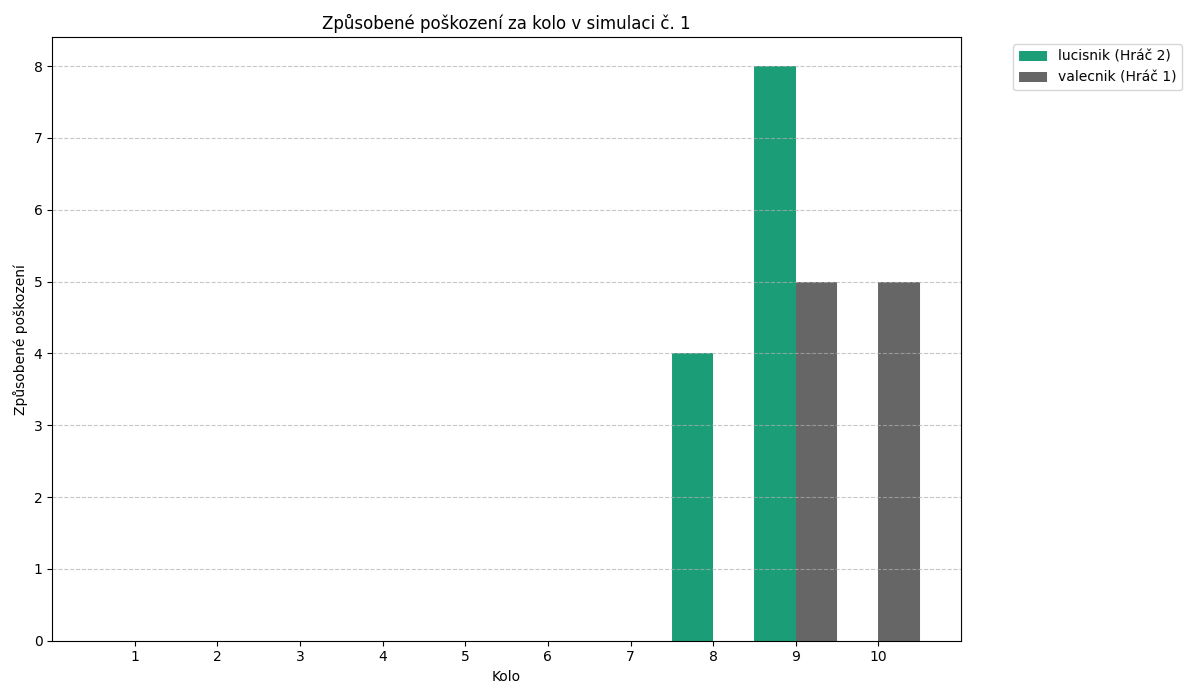
\includegraphics[scale=0.5]{obr/graf_valVSluc_flat_damage.png} % soubor + měřítko (scale)
  \caption{Graf poškození které jednotky způsobili v každém kole simulace} % popis obrázku
  \label{graf_valVSluc_flat_damage} % definice odkazu na obrázek (pro \ref{})
\end{figure}

\begin{figure}
  \centering      % vycentrovat
  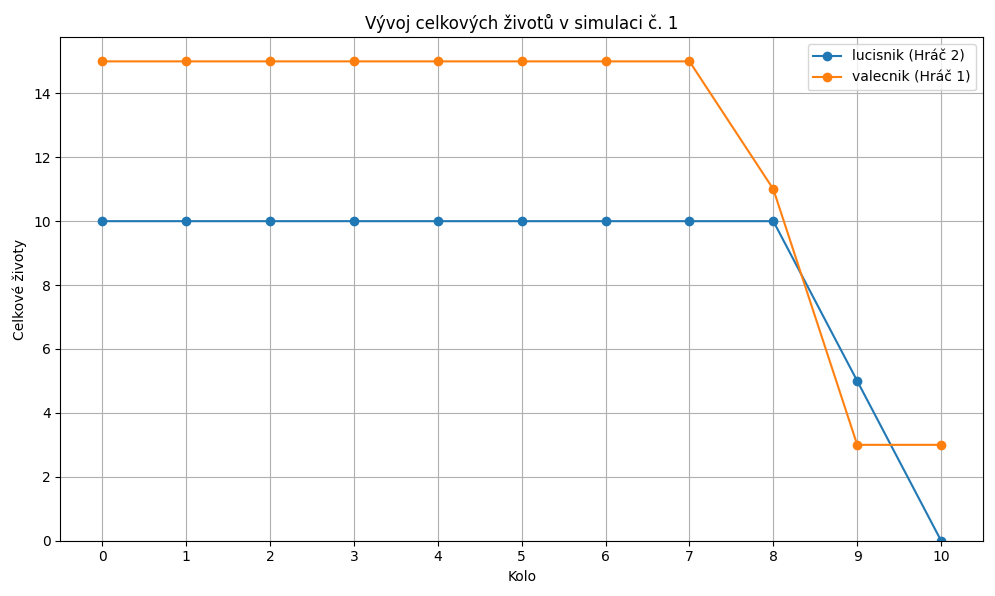
\includegraphics[scale=0.5]{obr/graf_valVSluc_flat_HP.png} % soubor + měřítko (scale)
  \caption{Graf životů jednotek v průběhu simulace} % popis obrázku
  \label{graf_valVSluc_flat_HP} % definice odkazu na obrázek (pro \ref{})
\end{figure}

\textbf{Analýza dat a interpretace:}

Průměrná délka souboje se oproti Linii prodloužila na 10 kol. Toto prodloužení souboje bylo zřejmě způsobeno tím, že jednotkám déle trvalo k sobě dojít, což jsem očekával, že bude zvýhodňovat lučištníka. K tomu nedošlo. Na grafech \ref{graf_valVSluc_flat_HP} a \ref{graf_valVSluc_flat_damage} je evidentně vidět, že jediná zásadní změna v tomto scénáři je delší doba, než se jednotky potkaly.

Tato simulace tedy nepřinesla žádné zásadní nové informace. Mohl bych zkusit lučištníka ještě trochu posílit, aby byl souboj ještě vyrovnanější, na druhou stranu je ale také pravda, že s lučištníkem se dají provádět strategické manévry, kterých prototypová AI není schopná, zkusím tedy atributy ponechat tak, jak jsou, a simulovat souboj v komplexnějším terénu.

\paragraph{Pohoří}~ \newline

\textbf{Počáteční atributy:}
\begin{itemize}
\item \textbf{Jednotka A (Válečník):} Útok:~8, Obrana:~4, Životy:~15, Rychlost:~3, Dosah:~1, \\ Cena (jídlo/dřevo/kámen):~60/30/0
\item \textbf{Jednotka B (Lučištník):} Útok:~8, Obrana:~3, Životy:~10, Rychlost:~3, Dosah:~4, \\ Cena (jídlo/dřevo/kámen):~15/15/0
\end{itemize}

\textbf{Výsledky simulace (agregace 10 simulací):}
\begin{itemize}
\item \textbf{Poměr vítězství:} Lučištník: 100\% simulací, Válečník: 0\% simulací.
\item \textbf{Průměrný počet kol:} 11.00
\item \textbf{Průměrné způsobené poškození za kolo (Válečník):} 0.55
\item \textbf{Průměrný počet útoků za kolo (Válečník):} 0.18
\item \textbf{Průměrná míra přežití (Válečník):} 0.00\%
\item \textbf{Průměrné způsobené poškození za kolo (Lučištník):} 1.45
\item \textbf{Průměrný počet útoků za kolo (Lučištník):} 0.55
\item \textbf{Průměrný počet protiútoků za kolo (Lučištník):} 0.18
\item \textbf{Průměrná míra přežití (Lučištník):} 100.00\%
\end{itemize}

\begin{figure}
  \centering      % vycentrovat
  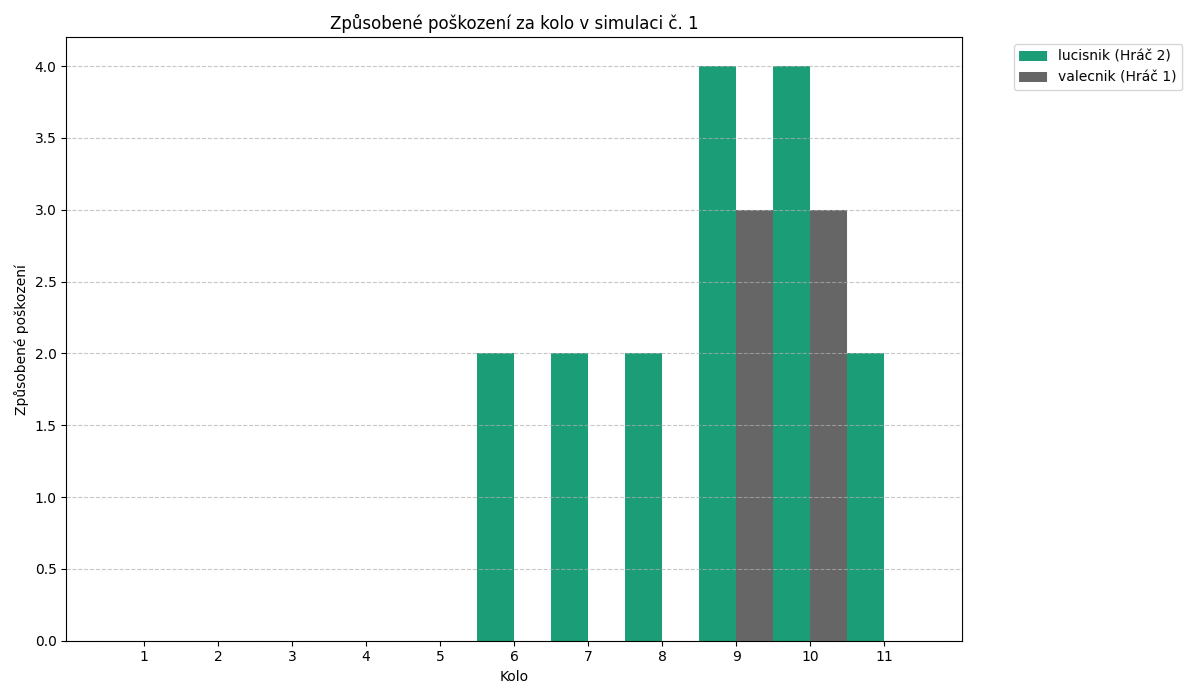
\includegraphics[scale=0.5]{obr/graf_valVSluc_nonflat_damage.png} % soubor + měřítko (scale)
  \caption{Graf poškození které jednotky způsobili v každém kole simulace} % popis obrázku
  \label{graf_valVSluc_nonflat_damage} % definice odkazu na obrázek (pro \ref{})
\end{figure}

\begin{figure}
  \centering      % vycentrovat
  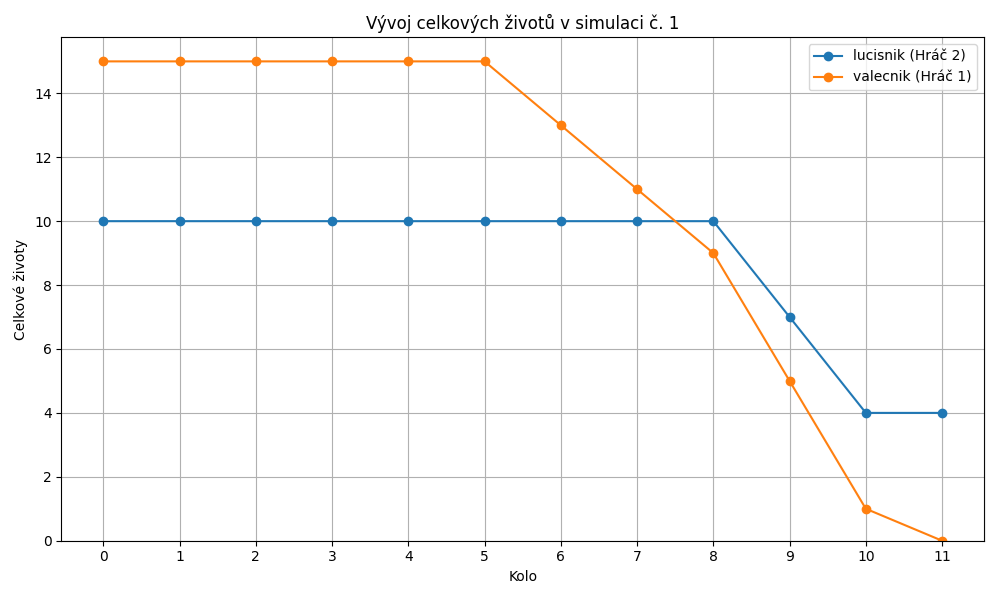
\includegraphics[scale=0.5]{obr/graf_valVSluc_nonflat_HP.png} % soubor + měřítko (scale)
  \caption{Graf životů jednotek v průběhu simulace} % popis obrázku
  \label{graf_valVSluc_nonflat_HP} % definice odkazu na obrázek (pro \ref{})
\end{figure}

\textbf{Analýza dat a interpretace:}

Průměrná délka souboje se prodloužila jen o jedno kolo, což je vzhledem k množství překážek překvapivé. Hory a lesy zpomalující pohyb válečníka, ale nepřekvapivě zásadně pomohli lučištníkovi způsobit dostatečné poškození, ačkoliv byl souboj těsný, lučištník tentokrát vyhrál.

V grafu poškození \ref{graf_valVSluc_nonflat_damage} je vidět, že celý souboj se odehrával v horách, kde je pohyb všech jednotek snížen na minimum, ale zároveň získávají jednotky bonus $+2$ k obraně. 

Z grafu životů \ref{graf_valVSluc_nonflat_HP} je pak vidět, že souboj byl těsný, lučištník už by další útok válečníka nepřežil, tedy prohlašuji jednotky za vyvážené.

\subsubsection{Rytíř vs. Berserkr}

\paragraph{Rovná linie}

\paragraph{Rovina}

\paragraph{Pohoří}

\subsubsection{Rytíř vs. Ostrostřelec}

\paragraph{Rovná linie}

\paragraph{Rovina}

\paragraph{Pohoří}

\subsubsection{Rytíř vs. Lovec}

\paragraph{Rovná linie}

\paragraph{Rovina}

\paragraph{Pohoří}

\subsubsection{Berserkr vs. Ostrostřelec}

\paragraph{Rovná linie}

\paragraph{Rovina}

\paragraph{Pohoří}

\subsubsection{Berserkr vs. Lovec}

\paragraph{Rovná linie}

\paragraph{Rovina}

\paragraph{Pohoří}

\subsubsection{Ostrostřelec vs. Lovec}

\paragraph{Rovná linie}

\paragraph{Rovina}

\paragraph{Pohoří}

\subsection{Fáze 1: Souboj více jednotek}


\chapter*{Závěr}
\addcontentsline{toc}{chapter}{Závěr} % SEM NESAHEJTE!
%
Zde napište text závěru (1-3 strany, nerozdělujte na podkapitoly) nebo jej vložte ze samostatného souboru: např. příkazem \texttt{\textbackslash input\{zaver.tex\}}.
%
%\input{zaver.tex}


%%%%%%%%%%%% SEZNAM POUŽITÝCH ZDROJŮ (LITERATURA) %%%%%%%%%%%%
%\addcontentsline{toc}{chapter}{Literatura} % SEM NESAHEJTE!
%\begin{thebibliography}{99}   
%	\bibitem{odkaz} Autor. \ti{Název knihy}. Město. Nakladatelství. Rok.  
%\end{thebibliography}
% formát: ČSN ISO 690. Můžete si to vygenerovat na http://www.citacepro.com (přihlaste se přes odkaz "ČVUT"), umí to vygenerovat TeX
% řazení: abecedně podle autora (resp. provního slova, není-li znám autor)

\addcontentsline{toc}{chapter}{Literatura} % SEM NESAHEJTE!
\begin{thebibliography}{99}   
% OBECNÉ PCG
	\bibitem{PCGinG}
    SHAKER, Noor; TOGELIUS, Julian a NELSON, Mark J. \textit{Procedural Content Generation in Games}. Switzerland: Springer International Publishing, 2016. ISBN 978-3-319-42714-0.
%file:///C:/Users/stepa/Downloads/978-3-319-42716-4%20(1).pdf

    \bibitem{HistoryOfPCG}
    SMITH, Gillian. \textit{An Analog History of Procedural Content Generation}. Paper. 360 Huntington Ave, 100 ME Boston, MA 02115, USA: Northeastern University, 2015.
%http://www.fdg2015.org/papers/fdg2015_paper_19.pdf

    \bibitem{PCGclanek}
    ANTONIOS LIAPIS. \textit{Constructive Generation Methods for Dungeons and Levels}. Online. Antoniosliapis.com. 2017. Dostupné z: \url{https://antoniosliapis.com/articles/pcgbook\_dungeons.php}. [cit. 2025-01-13].
%--------------------------------------------------

    \bibitem{BSPclanek}
    GEEKS FOR GEEKS. \textit{Binary Space Partitioning}. Online. Www.geeksforgeeks.org. 2020, 30 Sep, 2020. Dostupné z: \url{https://www.geeksforgeeks.org/binary-space-partitioning/}. [cit. 2025-01-13].

%--------------------------------------------------
% Agent-based

    \bibitem{Agent-basedClanek}
    DORAN, Jonathon a PARBERRY, Ian. Controlled Procedural Terrain Generation Using Software Agents. \textit{ReasearchGate}. 2010, vol.~2, no. 2, s.~111 - 119.
    %https://www.researchgate.net/publication/224133576_Controlled_Procedural_Terrain_Generation_Using_Software_Agents
%--------------------------------------------------
% Grammars
    %https://essay.utwente.nl/87002/
    \bibitem{GramClanek}
    \textit{Procedural Location Generation with Weighted Attribute Grammars}. Bakalářská práce. University of Twente P.O. Box 217, 7500AE Enschede The Netherlands: University of Twente, 2021.

    \bibitem{GramFand}
    \textit{Generative Grammars}. Online. Fandom.com. 2016. Dostupné z: \url{https://procedural-content-generation.fandom.com/wiki/Generative\_Grammars}. [cit. 2025-01-15].
%--------------------------------------------------
% Šum
    \bibitem{NoiseClanek}
    Travall. \textit{Procedural 2D Island Generation - Noise Functions}. Online. Https://medium.com. 2018. Dostupné z: \url{https://medium.com/@travall/procedural-2d-island-generation-noise-functions-13976bddeaf9}. [cit. 2025-01-16].

    \bibitem{perlinClanek}
    \textit{Perlin Noise}. Online. Scratchapixel.com. 2022. Dostupné z: \url{https://www.scratchapixel.com/lessons/procedural-generation-virtual-worlds/perlin-noise-part-2/perlin-noise.html}. [cit. 2025-01-16].

    %https://procedural-content-generation.fandom.com/wiki/Procedural_Content_Generation_Wiki
%--------------------------------------------------

    \bibitem{fracMath}
    BROWN, Adam. \textit{The Maths of Fractal Landscapes and Procedural Landscape Generation}. Online. Fractal-landscapes.co.uk. 2002 - 2020. Dostupné z: \url{https://www.fractal-landscapes.co.uk/maths.html}. [cit. 2025-01-16].

    \bibitem{waveClanek}
    HEATON, Robert. \textit{The Wavefunction Collapse Algorithm explained very clearly}. Online. Robertheaton.com. 17 Dec 2018. Dostupné z: \url{https://robertheaton.com/2018/12/17/wavefunction-collapse-algorithm/}. [cit. 2025-01-16].

    \bibitem{GANclanek}
    SPICK, Ryan J.; COWLING, Peter a WALKER, James Alfred. \textit{Procedural Generation using Spatial GANs for Region-Specific Learning of Elevation Data}. Paper. University of York, UK: University of York, 2019.

    \bibitem{navrh_level}
    ROGERS, Scott. \textit{Level UP! The guide to great video game design}. John Wiley \& Sons, 2010. ISBN 978-0-470-68867-0.
    
    \bibitem{navrh_rules}
    SALEN, Katie a ZIMMERMAN, Eric. \textit{Rules of Play - Game Design Fundamentals}. 2. Massachusetts Institute of Technology, 2004. ISBN 0-262-24045-9.
    
    \bibitem{navrh_lenses}
    SCHELL, Jesse. \textit{The art of game design: a book of lenses}. Boca Raton : CRC Press, 2008. ISBN 978-0-12-369496-6.


    
\end{thebibliography}

%%%%%%%%%%%% PŘÍLOHY PRÁCE %%%%%%%%%%%%
\newpage % SEM NESAHEJTE!
\addcontentsline{toc}{chapter}{Přílohy} % SEM NESAHEJTE!
\appendix % SEM NESAHEJTE!


%%%%%%%%%%%% Příloha A (tj. 1. kapitola v rámci příloh) %%%%%%%%%%%%
\chapter{Název přílohy} % SEM NESAHEJTE!
%
Zde napište text první přílohy nebo jej vložte, např.: \texttt{\textbackslash input\{priloha\_A.tex\}}.
%
%\input{priloha_A.tex} % text vkládán ze souboru, kde je i příkaz \chapter{...}


\end{document} % SEM NESAHEJTE! Konec.
